%%% Build instructions
%%% pdflatex -shell-escape ceres && bibtex ceres && pdflatex -shell-escape ceres && pdflatex -shell-escape ceres

\documentclass[10pt,letterpaper,oneside]{memoir}
\usepackage{fouriernc}
\usepackage[T1]{fontenc}
\usepackage{minted,amsmath,amssymb,amsthm,url,booktabs}
\usepackage[pdftex]{graphicx}
\usepackage[sort&compress]{natbib}
\usepackage[breaklinks=true,letterpaper=true,colorlinks,bookmarks=false]{hyperref}
\usepackage{algorithm}
\usepackage{algorithmic}

% page dimensions
\addtolength{\textwidth}{1.5in}
\addtolength{\oddsidemargin}{-0.75in}
\addtolength{\evensidemargin}{-0.75in}
\addtolength{\spinemargin}{-0.75in}
\addtolength{\foremargin}{-0.75in}
\setlength{\parindent}{0.0in}
\setlength{\parskip}{0.12in}

% Our pagestyle
\copypagestyle{ceres}{headings}
\makeevenhead{ceres}{\thepage}{}{\scshape\rightmark}
\makeoddhead{ceres}{\scshape\rightmark}{}{\thepage}

%% ceres chapter style
\makechapterstyle{ceres}{%
\renewcommand{\chapterheadstart}{}%
\renewcommand{\printchaptername}{}%
\renewcommand{\chapternamenum}{}%
\renewcommand{\printchapternum}{}%
\renewcommand{\afterchapternum}{}%
\renewcommand{\printchaptertitle}[1]{%
\raggedright\Large\scshape\MakeLowercase{##1}}%
\renewcommand{\afterchaptertitle}{%
\vskip\onelineskip \hrule\vskip\onelineskip}%
}%
\renewcommand{\cftchapterfont}{\normalfont}%
\renewcommand{\cftchapterpagefont}{\normalfont}%
\renewcommand{\cftchapterpresnum}{\bfseries}%
\renewcommand{\cftchapterleader}{}%
\renewcommand{\cftchapterafterpnum}{\cftparfillskip}%


%% Section title style
\setsecheadstyle{\raggedright\scshape\MakeLowercase}%
\setbeforesecskip{-\onelineskip}%
\setaftersecskip{\onelineskip}%

%% Subsection title style

\setsubsecheadstyle{\sethangfrom{\noindent ##1}\raggedright\itshape}%
\setbeforesubsecskip{-\onelineskip}%
\setaftersubsecskip{\onelineskip}%

\captiontitlefont{\small\sffamily}%
\let\caption\legend


\title{\Huge\scshape
\MakeLowercase{Ceres Solver:  Tutorial \& Reference}
}
\author{
\scshape\MakeLowercase{Sameer Agarwal} \\ \texttt{sameeragarwal@google.com}
\and
\scshape\MakeLowercase{Keir Mierle} \\  \texttt{ mierle@gmail.com}
}
\checkandfixthelayout

\pagestyle{ceres}

\newcommand{\ceres}{{Ceres }}
\newcommand{\reals}{\mathbb{R} }
\def\eg{\emph{e.g. }}
\def\ie{\emph{i.e. }}
\newcommand{\glog}{\texttt{google-glog}}
\newcommand{\gflags}{\texttt{gflags}}
\newcommand{\eigen}{\texttt{Eigen3}}
\newcommand{\suitesparse}{\texttt{SuiteSparse}}
\newcommand{\cholmod}{\texttt{CHOLMOD}}
\newcommand{\amd}{\texttt{AMD}}
\newcommand{\colamd}{\texttt{COLAMD}}
\newcommand{\lapack}{\texttt{LAPACK}}
\newcommand{\blas}{\texttt{BLAS}}
\newcommand{\denseschur}{\texttt{DENSE\_SCHUR}}
\newcommand{\sparseschur}{\texttt{SPARSE\_SCHUR}}
\newcommand{\iterativeschur}{\texttt{ITERATIVE\_SCHUR}}
\newcommand{\cmake}{\texttt{cmake}}
\newcommand{\protobuf}{\texttt{protobuf}}
\settocdepth{chapter}

\begin{document}
\chapterstyle{ceres}
\maketitle
\thispagestyle{empty}
\newpage
\pagestyle{ceres}
\tableofcontents
\newpage

\chapter{A Note to the Reader}
Building this pdf from source requires a relatively recent installation of \texttt{LaTeX}~\footnote{\url{http://www.tug.org/texlive/}}, \texttt{minted.sty}\footnote{\url{http://code.google.com/p/minted/}} and \texttt{pygments}\footnote{\url{http://pygments.org/}}.

Despite our best efforts, this manual remains a work in progress and the source code for Ceres Solver remains the ultimate reference.
%!TEX root = ceres-solver.tex

\chapter{Version History}
\section*{1.3.0}
\subsection{New Features}
\begin{itemize}
\item Windows port. (Changchang Wu and Pierre Moulon also contributed to the port)
\item Support for returning initial and final derivatives (Gradient \& Jacobian).
\item Gradient computation support in the evaluators, with an eye towards developing first order/gradient based solvers.
\item Ability to build Ceres as a shared library, associated versioning and build release script changes.
\item A better way to compute \texttt{Solver::Summary::fixed\_cost}. (Markus Moll)
\item Portable floating point classification API.
\end{itemize}

\subsection{Bug Fixes}
\begin{itemize}
\item Fix IsInfinite on Jets.
\item Drop alignment requirements for Jets.
\item Fixed Jet to integer comparison. (Keith Leung)
\item Fix use of uninitialized arrays. (Sebastian Koch \& Markus Moll)
\item Conditionally compile gflag dependencies.(Casey Goodlett)
\item Add \texttt{data\_fitting.cc } to the examples CMake file.
\end{itemize}

\section*{1.2.3}
\subsection{Bug Fixes}
\begin{itemize}
\item \texttt{suitesparse\_test} is enabled even when \texttt{-DSUITESPARSE=OFF}.
\item \texttt{FixedArray} internal struct did not respect \texttt{Eigen}
  alignment requirements (Koichi Akabe \& Stephan Kassemeyer).
\item Fixed \texttt{quadratic.cc} documentation and code mismatch
  (Nick Lewycky).
\end{itemize}
\section*{1.2.2}
\subsection{Bug Fixes}
\begin{itemize}
\item Fix constant parameter blocks, and other minor fixes (Markus Moll)
\item Fix alignment issues when combining \texttt{Jet} and
  \texttt{FixedArray} in automatic differeniation.
\item Remove obsolete \texttt{build\_defs} file.
\end{itemize}
\section*{1.2.1}
\subsection{New Features}
\begin{itemize}
\item Powell's Dogleg solver
\item Documentation now has a brief overview of Trust Region methods and how the Levenberg-Marquardt and Dogleg methods work.
\end{itemize}
\subsection{Bug Fixes}
\begin{itemize}
\item Destructor for \texttt{TrustRegionStrategy} was not virtual (Markus Moll)
\item Invalid \texttt{DCHECK} in \texttt{suitesparse.cc} (Markus Moll)
\item Iteration callbacks were not properly invoked (Luis Alberto Zarrabeiti)
\item Logging level changes in ConjugateGradientsSolver
\item VisibilityBasedPreconditioner setup does not account for skipped camera pairs. This was debugging code.
\item Enable SSE support on MacOS
\item \texttt{system\_test} was taking too long and too much memory (Koichi Akabe)
\end{itemize}
\section*{1.2.0}
\subsection{New Features}
\begin{itemize}
\item \texttt{CXSparse} support.
\item Block oriented fill reducing orderings. This
reduces the factorization time for sparse
\texttt{CHOLMOD} significantly.
\item New Trust region loop with support for multiple
trust region step strategies. Currently only Levenberg-Marquardt is supported, but this refactoring opens the door for Dog-leg, Stiehaug and others.
\item \texttt{Cmake} file restructuring.  Builds in \texttt{Release} mode by default, and now has platform specific tuning flags.
\item Re-organized documentation. No new content, but better organization.
\end{itemize}

\subsection{Bug Fixes}
\begin{itemize}
\item Fixed integer overflow bug in \texttt{block\_random\_access\_sparse\_matrix.cc}.
\item Renamed some macros to prevent name conflicts.
\item Fixed incorrent input to \texttt{StateUpdatingCallback}.
\item Fixes to AutoDiff tests.
\item Various internal cleanups.
\end{itemize}

\section*{1.1.1}
\subsection{Bug Fixes}
\begin{itemize}
\item Fix a bug in the handling of constant blocks. (Louis Simard)
\item Add an optional lower bound to the Levenberg-Marquardt regularizer to prevent oscillating between well and ill posed linear problems.
\item Some internal refactoring and test fixes.
\end{itemize}
\section{1.1.0}
\subsection{New Features}
\begin{itemize}
\item New iterative linear solver for general sparse problems - \texttt{CGNR} and a block Jacobi preconditioner for it.
\item Changed the semantics of how \texttt{SuiteSparse} dependencies are checked and used. Now \texttt{SuiteSparse} is built by default, only if all of its dependencies are present.
\item Automatic differentiation now supports dynamic number of residuals.
\item Support for writing the linear least squares problems to disk in text format so that they can loaded into \texttt{MATLAB}.
\item Linear solver results are now checked for nan and infinities.
\item Added \texttt{.gitignore} file.
\item A better more robust build system.
\end{itemize}

\subsection{Bug Fixes}
\begin{itemize}
\item Fixed a strict weak ordering bug in the schur ordering.
\item Grammar and typos in the documents and code comments.
\item Fixed tests which depended on exact equality between floating point values.
\end{itemize}
\section*{1.0.0}
Initial Release.

%!TEX root = ceres-solver.tex
\chapter{Introduction}
\label{chapter:introduction}
Ceres Solver\footnote{For brevity, in the rest of this document we will just use the term Ceres.} is a non-linear least squares solver developed at Google. It is designed to solve small and large sparse problems accurately and efficiently~\footnote{For a gentle but brief introduction to non-liner least squares problems, please start by reading the~\hyperref[part:tutorial]{Tutorial}}. Amongst its various features is a simple but expressive API with support for automatic differentiation, robust norms, local parameterizations, automatic gradient checking, multithreading and automatic problem structure detection.

The key computational cost when solving a non-linear least squares problem is the solution of a linear least squares problem in each iteration. To this end Ceres supports a number of different linear solvers suited for different needs. This includes dense QR factorization (using \eigen) for small scale problems, sparse Cholesky factorization (using \texttt{SuiteSparse}) for general sparse problems and specialized Schur complement based solvers for problems that arise in multi-view geometry~\cite{hartley-zisserman-book-2004}.

Ceres has been used for solving a variety of problems in computer vision and machine learning at Google with sizes that range from a tens of variables and objective functions with a few hundred terms to problems with millions of variables and objective functions with tens of millions of terms. 


\section{What's in a name?}
While there is some debate as to who invented of the method of Least Squares~\cite{stigler1981gauss}. There is no debate that it was Carl Friedrich Gauss's prediction of the orbit of the newly discovered asteroid Ceres based on just 41 days of observations that brought it to the attention of the world~\cite{tennenbaum-director}. We named our solver after Ceres to celebrate this seminal event in the history of astronomy, statistics and optimization.

\section{Contributing to Ceres Solver}

We welcome contributions to Ceres, whether they are new features, bug fixes or tests. The Ceres mailing list\footnote{\url{http://groups.google.com/group/ceres-solver}} is the best place for all development related discussions. Please consider joining it. If you have ideas on how you would like to contribute to Ceres, it is a good idea to let us know on the mailinglist before you start development. We may have suggestions that will save effort when trying to merge your work into the main branch. If you are looking for ideas, please let us know about your interest and skills and we will be happy to make a suggestion or three.

We follow Google's C++ Style Guide~\footnote{\url{http://google-styleguide.googlecode.com/svn/trunk/cppguide.xml}} and use \texttt{git} for version control.

\section{Citing Ceres Solver}
If you use Ceres for an academic publication, please cite this manual. e.g.,
\begin{verbatim}
@manual{ceres-manual,
	Author = {Sameer Agarwal and Keir Mierle},
	Title = {Ceres Solver: Tutorial \& Reference},
	Organization = {Google Inc.}
}
\end{verbatim}
	

\section{Acknowledgements}
A number of people have helped with the development and open sourcing of Ceres. 

Fredrik Schaffalitzky when he was at Google started the development of Ceres, and even though much has changed since then, many of the ideas from his original design are still present in the current code.

Amongst Ceres' users at Google two deserve special mention: William Rucklidge and James Roseborough. William was the first user of Ceres. He bravely took on the task of porting production code to an as-yet unproven optimization library, reporting bugs and helping fix them along the way. James is perhaps the most sophisticated user of Ceres at Google. He has reported and fixed bugs and helped evolve the API for the better.

Nathan Wiegand contributed the MacOS port.



%!TEX root = ceres-solver.tex
\chapter{License}
Ceres Solver is licensed under the New BSD license, whose terms are as follows.

\begin{quotation}

\noindent
Copyright (c) 2010, 2011, 2012, Google Inc. All rights reserved.

\noindent
Redistribution and use in source and binary forms, with or without
modification, are permitted provided that the following conditions are met:
\begin{enumerate}
\item Redistributions of source code must retain the above copyright notice,
      this list of conditions and the following disclaimer.
\item Redistributions in binary form must reproduce the above copyright notice,
      this list of conditions and the following disclaimer in the documentation
      and/or other materials provided with the distribution.
\item Neither the name of Google Inc.,  nor the names of its contributors may
      be used to endorse or promote products derived from this software without
      specific prior written permission.
\end{enumerate}

\noindent
This software is provided by the copyright holders and contributors "AS IS" and
any express or implied warranties, including, but not limited to, the implied
warranties of merchantability and fitness for a particular purpose are
disclaimed. In no event shall Google Inc. be liable for any direct, indirect,
incidental, special, exemplary, or consequential damages (including, but not
limited to, procurement of substitute goods or services; loss of use, data, or
profits; or business interruption) however caused and on any theory of
liability, whether in contract, strict liability, or tort (including negligence
or otherwise) arising in any way out of the use of this software, even if
advised of the possibility of such damage.
\end{quotation}

%!TEX root = ceres-solver.tex
\chapter{Building Ceres}
\label{chapter:build}
Ceres source code and documentation are hosted at
\url{http://code.google.com/p/ceres-solver/}.

\section{Dependencies}
Ceres relies on a number of open source libraries, some of which are optional. For details on customizing the build process, please see Section~\ref{sec:custom}.

\begin{enumerate}
\item{\cmake~\footnote{\url{http://www.cmake.org/}}} is the cross-platform build system used by Ceres. We require that you have a relative recent install of \texttt{cmake} (version 2.8.0 or better).
\item{\eigen~\footnote{\url{http://eigen.tuxfamily.org}}} is used for doing all the low level matrix and
  linear algebra operations.

\item{\glog~\footnote{\url{http://code.google.com/p/google-glog}}} is used for error checking and logging.

 Note: Ceres requires \texttt{glog}\ version 0.3.1 or later. Version 0.3 (which ships with Fedora 16) has a namespace bug which prevents Ceres from building.

\item{\gflags~\footnote{\url{http://code.google.com/p/gflags}}} is used by the code in
  \texttt{examples}. It is also used by some of the tests. Strictly speaking it is not required to build the core library, \textbf{ we do not recommend building Ceres without \texttt{gflags}}.

\item{\suitesparse~\footnote{\url{http://www.cise.ufl.edu/research/sparse/SuiteSparse/}}} is used for sparse matrix analysis,
  ordering and factorization. In particular Ceres uses the
  \amd, \colamd\ and \cholmod\ libraries. This is an optional
  dependency.

\item{\texttt{CXSparse}~\footnote{\url{http://www.cise.ufl.edu/research/sparse/CXSparse/}}} is used for sparse matrix analysis, ordering and factorization. While it is similar to \texttt{SuiteSparse} in scope, its performance is a bit worse but is a much simpler library to build and does not have any other dependencies. This is an optional dependency.

\item{\blas\ and \lapack} are needed by
  \suitesparse.  We
  recommend either
  \texttt{GotoBlas2}~\footnote{\url{http://www.tacc.utexas.edu/tacc-projects/gotoblas2}}
  or
  \texttt{ATLAS}~\footnote{\url{http://math-atlas.sourceforge.net/}},
    both of which ship with \blas\ and \lapack\ routines.

\item{\texttt{protobuf}~\footnote{\url{http://code.google.com/p/protobuf/}}} is an optional dependency that is used for serializing and deserializing linear least squares problems to disk. This is useful for debugging and testing. Without it, some of the tests will be disabled.
\end{enumerate}

Currently we support building on Linux and MacOS X. Support for other
platforms is forthcoming.

\section{Building on Linux}
We will use Ubuntu as our example platform.

\begin{enumerate}
\item{\cmake}
\begin{minted}{bash}
sudo apt-get install cmake
\end{minted}

\item{\gflags} can either be installed from source via the \texttt{autoconf} invocation
\begin{minted}{bash}
tar -xvzf gflags-2.0.tar.gz
cd gflags-2.0
./configure --prefix=/usr/local
make
sudo make install.
\end{minted}
or via the \texttt{deb} or \texttt{rpm} packages available on the \gflags\ website.

\item{\glog} must be configured to use the previously installed
\gflags, rather than the stripped down version that is bundled with \glog. Assuming you have it installed in \texttt{/usr/local} the following \texttt{autoconf} invocation installs it.
\begin{minted}{bash}
tar -xvzf glog-0.3.2.tar.gz
cd glog-0.3.2
./configure --with-gflags=/usr/local/
make
sudo make install
\end{minted}

\item{\eigen}
\begin{minted}{bash}
sudo apt-get install libeigen3-dev
\end{minted}

\item{\suitesparse\ and \texttt{CXSparse}}
\begin{minted}{bash}
sudo apt-get install libsuitesparse-dev
\end{minted}
This should automatically bring in the necessary \blas\ and \lapack\ dependencies. By co-incidence on Ubuntu, this also installs \texttt{CXSparse}.

\item{\texttt{protobuf}}
\begin{minted}{bash}
sudo apt-get install libprotobuf-dev
\end{minted}
\end{enumerate}


We are now ready to build and test Ceres. Note that \texttt{cmake} requires the exact path to the \texttt{libglog.a} and \texttt{libgflag.a}

\begin{minted}{bash}
tar zxf ceres-solver-1.2.1.tar.gz
mkdir ceres-bin
cd ceres-bin
cmake ../ceres-solver-1.2.1
make -j3
make test
\end{minted}

You can also try running the command line bundling application with one of the
included problems, which comes from the University of Washington's BAL dataset~\cite{Agarwal10bal}:
\begin{minted}{bash}
bin/simple_bundle_adjuster \
  ../ceres-solver-1.2.1/data/problem-16-22106-pre.txt \
\end{minted}
This runs Ceres for a maximum of 10 iterations using the  \denseschur\ linear solver. The output should look something like this.
\clearpage
\begin{minted}{bash}
0: f: 1.598216e+06 d: 0.00e+00 g: 5.67e+18 h: 0.00e+00 rho: 0.00e+00 mu: 1.00e-04 li:  0
1: f: 1.116401e+05 d: 1.49e+06 g: 1.42e+18 h: 5.48e+02 rho: 9.50e-01 mu: 3.33e-05 li:  1
2: f: 4.923547e+04 d: 6.24e+04 g: 8.57e+17 h: 3.21e+02 rho: 6.79e-01 mu: 3.18e-05 li:  1
3: f: 1.884538e+04 d: 3.04e+04 g: 1.45e+17 h: 1.25e+02 rho: 9.81e-01 mu: 1.06e-05 li:  1
4: f: 1.807384e+04 d: 7.72e+02 g: 3.88e+16 h: 6.23e+01 rho: 9.57e-01 mu: 3.53e-06 li:  1
5: f: 1.803397e+04 d: 3.99e+01 g: 1.35e+15 h: 1.16e+01 rho: 9.99e-01 mu: 1.18e-06 li:  1
6: f: 1.803390e+04 d: 6.16e-02 g: 6.69e+12 h: 7.31e-01 rho: 1.00e+00 mu: 3.93e-07 li:  1

Ceres Solver Report
-------------------
                                     Original                  Reduced
Parameter blocks                        22122                    22122
Parameters                              66462                    66462
Residual blocks                         83718                    83718
Residual                               167436                   167436

                                        Given                     Used
Linear solver                     DENSE_SCHUR              DENSE_SCHUR
Preconditioner                            N/A                      N/A
Ordering                                SCHUR                    SCHUR
num_eliminate_blocks                      N/A                    22106
Threads:                                    1                        1
Linear Solver Threads:                      1                        1

Cost:
Initial                          1.598216e+06
Final                            1.803390e+04
Change                           1.580182e+06

Number of iterations:
Successful                                  6
Unsuccessful                                0
Total                                       6

Time (in seconds):
Preprocessor                     0.000000e+00
Minimizer                        2.000000e+00
Total                            2.000000e+00
Termination:               FUNCTION_TOLERANCE
\end{minted}

\section{Building on OS X}
On OS X, we recommend using the \texttt{homebrew}~\footnote{\url{http://mxcl.github.com/homebrew/}} package manager.

\begin{enumerate}
\item{\cmake}
\begin{minted}{bash}
brew install cmake
\end{minted}
\item{\texttt{glog}\ and \texttt{gflags}}

Installing \texttt{\glog} takes also brings in \texttt{gflags} as a dependency.
\begin{minted}{bash}
brew install glog
\end{minted}
\item{\eigen}
\begin{minted}{bash}
brew install eigen
\end{minted}
\item{\suitesparse\ and \texttt{CXSparse}}
\begin{minted}{bash}
brew install suite-sparse
\end{minted}
\item{\texttt{protobuf}}
\begin{minted}{bash}
brew install protobuf
\end{minted}
\end{enumerate}

We are now ready to build and test Ceres.
\begin{minted}{bash}
tar zxf ceres-solver-1.2.1.tar.gz
mkdir ceres-bin
cd ceres-bin
cmake ../ceres-solver-1.2.1
make -j3
make test
\end{minted}
Like the Linux build, you should now be able to run \texttt{bin/simple\_bundle\_adjuster}.


\section{Building on Windows with Visual Studio}
On Windows, we support building with Visual Studio 2010 or newer. Note that the
Windows port is less featureful and less tested than the Linux or Mac OS X
versions due to the unavaliability of SuiteSparse and CXSparse. Building is
also more involved since there is no automated way to install the dependencies.

\begin{enumerate}
  \item Make a toplevel directory for deps \& build \& src somewhere: \texttt{ceres/}
  \item Get dependencies; unpack them as subdirectories in \texttt{ceres/}
        (\texttt{ceres/eigen}, \texttt{ceres/glog}, etc)
        \begin{itemize}
          \item Eigen 3.1 from eigen.tuxfamily.org (needed on Windows; 3.0.x will not
                work). There is no need to build anything; just unpack the source
                tarball.
          \item Goolge Log. Open up the Visual Studio solution and build it.
          \item Goolge Flags. Open up the Visual Studio solution and build it.
        \end{itemize}
  \item Unpack the Ceres tarball into \texttt{ceres}. For the tarball, you
        should get a directory inside \texttt{ceres} similar to
        \texttt{ceres-solver-1.3.0}. Alternately, checkout Ceres via git to get
        \texttt{ceres-solver.git} inside \texttt{ceres}.
  \item Install CMake.
  \item Make a dir \texttt{ceres/ceres-bin} (for an out-of-tree build)
  \item Run CMake; select the \texttt{ceres-solver-X.Y.Z} or
        \texttt{ceres-solver.git} directory for the CMake file. Then select the
        \texttt{ceres-bin} for the build dir.
  \item Try running "Configure". It won't work. It'll show a bunch of options.
        You'll need to set:
        \begin{itemize}
        \item \texttt{GLOG\_INCLUDE}
        \item \texttt{GLOG\_LIB}
        \item \texttt{GFLAGS\_LIB}
        \item \texttt{GFLAGS\_INCLUDE}
        \end{itemize}
        to the appropriate place where you unpacked/built them.
  \item You may have to tweak some more settings to generate a MSVC project.
        After each adjustment, try pressing Configure \& Generate until it
        generates successfully.
  \item Open the solution and build it in MSVC
\end{enumerate}

To run the tests, select the \texttt{RUN\_TESTS} target and hit "Build RUN\_TESTS" from the build menu.

Like the Linux build, you should now be able to run \texttt{bin/simple\_bundle\_adjuster}.

Notes:
\begin{itemize}
\item The default build is Debug; consider switching it to release mode.
\item Currently \texttt{system\_test} is not working properly.
\item Building Ceres as a DLL is not supported; patches welcome.
\item CMake puts the resulting test binaries in ceres-bin/examples/Debug by
      default.
\item The solvers supported on Windows are \texttt{DENSE\_QR},
      \texttt{DENSE\_SCHUR}, \texttt{CGNR}, and \texttt{ITERATIVE\_SCHUR}.
\item We're looking for someone to work with upstream SuiteSparse to port their
      build system to something sane like CMake, and get a supported Windows
      port.
\end{itemize}

\section{Building on Android}
\label{sec:android}
Download the Android NDK. Run \texttt{ndk-build} from inside the \texttt{jni} directory. Use the \texttt{libceres.a} that gets created.

\section{Compiler Flags to use when building your own applications}
\label{sec:compiler-flags}
TBD


\section{Customizing the Build Process}
\label{sec:custom}
It is possible to reduce the libraries needed to build Ceres and
customize the build process by passing appropriate flags to \texttt{cmake}. But unless you really know what you are
doing, we recommend against disabling any of the following flags.

\begin{enumerate}
\item{\texttt{protobuf}}


Protocol Buffers is a big dependency and if you do not care for the tests that depend on it and the logging support it enables, you can turn it off by using
\begin{minted}{bash}
-DPROTOBUF=OFF.
\end{minted}

\item{\suitesparse}

By default, Ceres will only link to \texttt{SuiteSparse}\  if all its dependencies are present.
To build Ceres without \suitesparse\ use
\begin{minted}{bash}
-DSUITESPARSE=OFF.
\end{minted}
 This will also disable dependency checking for \lapack\ and \blas. This saves on binary size, but the resulting version of Ceres is not suited
to large scale problems due to the lack of a sparse Cholesky solver.  This will reduce Ceres' dependencies down to
\eigen, \gflags\ and \glog.

\item{\texttt{CXSparse}}

By default, Ceres will only link to \texttt{CXSparse} if all its dependencies are present.
To build Ceres without \suitesparse\ use
\begin{minted}{bash}
-DCXSPARSE=OFF.
\end{minted}

This saves on binary size, but the resulting version of Ceres is not suited to large scale problems due to the lack of a sparse Cholesky solver.  This will reduce Ceres' dependencies down to
\eigen, \gflags\ and \glog.

\item{\gflags}
To build Ceres without \gflags, use
\begin{minted}{bash}
-DGFLAGS=OFF.
\end{minted}
Disabling this flag will prevent some of the example code from building.

\item{Template Specializations}


If you are concerned about binary size/compilation time over some
small (10-20\%) performance gains in the \sparseschur\ solver, you can disable some of the template
specializations by using
\begin{minted}{bash}
-DSCHUR_SPECIALIZATIONS=OFF.
\end{minted}

\item{\texttt{OpenMP}}


On certain platforms like Android, multithreading with OpenMP is not supported. OpenMP support can be disabled by using
\begin{minted}{bash}
-DOPENMP=OFF.
\end{minted}
\end{enumerate}



%% Tutorial
\part{Tutorial}
\label{part:tutorial}
%!TEX root = ceres.tex
\chapter{Non-linear Least Squares}
\label{chapter:tutorial:nonlinsq}
Let $x \in \reals^n$ be an $n$-dimensional vector of variables, and
$F(x) = \left[f_1(x); \hdots ; f_k(x)\right]$ be a vector of residuals $f_i(x)$. 
The function $f_i(x)$ can be a scalar or a vector valued
function.  Then, 
\begin{equation}
	\arg \min_x \frac{1}{2} \sum_{i=1}^k \|f_i(x)\|^2.
\end{equation}
is a Non-linear Least Squares problem~\footnote{Ceres can solve a more general version of this problem, but for pedagogical reasons, we will restrict ourselves to this class of problems for now. See section~\ref{chapter:overview} for a full description of the problems that Ceres can solve}. Here $\|\cdot\|$ denotes the Euclidean norm of a vector. 

Such optimization problems arise in almost every area of science and engineering. Whenever there is data to be analyzed, curves to be fitted, there is usually a linear or a non-linear least squares problem lurking in there somewhere. 

Perhaps the simplest example of such a problem is the problem of Ordinary Linear Regression, where given observations $(x_1,y_1),\hdots, (x_k,y_k)$, we wish to find the line $y = mx + c$, that best explains $y$ as a function of $x$. One way to solve this problem is to find the solution to the following optimization problem
\begin{equation}
		\arg\min_{m,c} \sum_{i=1}^k (y_i - m x_i - c)^2.
\end{equation}
With a little bit of calculus, this problem can be solved easily by hand. But what if, instead of a line we were interested in a more complicated relationship between $x$ and $y$, say for example $y = e^{mx + c}$. Then the optimization problem becomes
\begin{equation}
		\arg\min_{m,c} \sum_{i=1}^k \left(y_i - e^{m x_i + c}\right)^2.
\end{equation}
This is a  non-linear regression problem and solving it by hand is much more tedious.  Ceres is designed to help you model and solve problems like this easily and efficiently.
%!TEX root = ceres-solver.tex
\chapter{Hello World!}
\label{chapter:tutorial:helloworld}
To get started, let us consider the problem of finding the minimum of the function
\begin{equation}
 \frac{1}{2}(10 -x)^2.
\end{equation}
This is a trivial problem, whose minimum is easy to see is located at $x = 10$, but it is a good place to start to illustrate the basics of solving a problem with Ceres\footnote{Full working code for this and other examples in this manual can be found in the \texttt{examples} directory. Code for this example can be found in \texttt{examples/quadratic.cc}}. 


Let us write this problem as a non-linear least squares problem by defining the scalar residual function $f_1(x) = 10 - x$. Then $F(x) = [f_1(x)]$ is a residual vector with exactly one component.

When solving a problem with Ceres, the first thing to do is to define a subclass of \texttt{CostFunction}. It is responsible for computing the value of the residual function and its derivative (also known as the Jacobian) with respect to $x$.
\begin{minted}[mathescape]{c++}
class SimpleCostFunction
  : public ceres::SizedCostFunction<1 /* number of residuals */,
                                    1 /* size of first parameter */> {
 public:
  virtual ~SimpleCostFunction() {}
  virtual bool Evaluate(double const* const* parameters,
                        double* residuals,
                        double** jacobians) const {
    const double x = parameters[0][0];
    residuals[0] = 10 - x;  // $f(x) = 10 - x$
    // Compute the Jacobian if asked for.
    if (jacobians != NULL && jacobians[0] != NULL) {
      jacobians[0][0] = -1;
    }
    return true;
  }
};
\end{minted}
\texttt{SimpleCostFunction} is provided with an input array of parameters, an output array for residuals and an optional output array for Jacobians. In our example, there is just one parameter and one residual and this is known at compile time, therefore we can save some code and instead of inheriting from \texttt{CostFunction}, we can instaed inherit from the templated \texttt{SizedCostFunction} class. 


The \texttt{jacobians} array is optional, \texttt{Evaluate} is expected to check when it is non-null, and if it is the case then fill it with the values of the derivative of the residual function. In this case since the residual function is linear, the Jacobian is constant.

Once we have a way of computing the residual vector, it is now time to construct a Non-linear least squares problem using it and have Ceres solve it.
\begin{minted}{c++}
int main(int argc, char** argv) {
  double x = 5.0;
  ceres::Problem problem;

  // The problem object takes ownership of the newly allocated
  // SimpleCostFunction and uses it to optimize the value of x.
  problem.AddResidualBlock(new SimpleCostFunction, NULL, &x);

  // Run the solver!
  Solver::Options options;
  options.max_num_iterations = 10;
  options.linear_solver_type = ceres::DENSE_QR;
  options.minimizer_progress_to_stdout = true;
  Solver::Summary summary;
  Solve(options, &problem, &summary);
  std::cout << summary.BriefReport() << "\n";
  std::cout << "x : 5.0 -> " << x << "\n";
  return 0;
}
\end{minted}

Compiling and running this program gives us
\begin{minted}{bash}
0: f: 1.250000e+01 d: 0.00e+00 g: 5.00e+00 h: 0.00e+00 rho: 0.00e+00 mu: 1.00e-04 li:  0
1: f: 1.249750e-07 d: 1.25e+01 g: 5.00e-04 h: 5.00e+00 rho: 1.00e+00 mu: 3.33e-05 li:  1
2: f: 1.388518e-16 d: 1.25e-07 g: 1.67e-08 h: 5.00e-04 rho: 1.00e+00 mu: 1.11e-05 li:  1
Ceres Solver Report: Iterations: 2, Initial cost: 1.250000e+01,  \
Final cost: 1.388518e-16, Termination: PARAMETER_TOLERANCE.
x : 5 -> 10
\end{minted}

Starting from a $x=5$, the solver in two iterations goes to 10~\footnote{Actually the solver ran for three iterations, and it was by looking at the value returned by the linear solver in the third iteration, it observed that the update to the parameter block was too small and declared convergence. Ceres only prints out the display at the end of an iteration, and terminates as soon as it detects convergence, which is why you only see two iterations here and not three.}. The careful reader will note that this is a linear problem and one linear solve should be enough to get the optimal value.  The default configuration of the solver is aimed at non-linear problems, and for reasons of simplicity we did not change it in this example. It is indeed possible to obtain the solution to this problem using Ceres in one iteration. Also note that the solver did get very close to the optimal function value of 0 in the very first iteration. We will discuss these issues in greater detail when we talk about convergence and parameter settings for Ceres.

%!TEX root = ceres-solver.tex
\chapter{Powell's Function}
\label{chapter:tutorial:powell}
Consider now a slightly more complicated example -- the minimization of Powell's function. Let $x = \left[x_1, x_2, x_3, x_4 \right]$ and
\begin{align}
   f_1(x) &= x_1 + 10*x_2 \\
   f_2(x) &= \sqrt{5} * (x_3 - x_4)\\
   f_3(x) &= (x_2 - 2*x_3)^2\\
   f_4(x) &= \sqrt{10} * (x_1 - x_4)^2\\
	F(x) & = \left[f_1(x),\ f_2(x),\ f_3(x),\ f_4(x) \right]
\end{align}
$F(x)$ is a function of four parameters, and has four residuals. Now,
one way to solve this problem would be to define four
\texttt{CostFunction} objects that compute the residual and Jacobians. \eg the following code shows the implementation for $f_4(x)$.
\begin{minted}[mathescape]{c++}
class F4 : public ceres::SizedCostFunction<1, 4> {
 public:
  virtual ~F4() {}
  virtual bool Evaluate(double const* const* parameters,
                        double* residuals,
                        double** jacobians) const {
    double x1 = parameters[0][0];
    double x4 = parameters[1][0];
    // $f_4 = \sqrt{10} * (x_1 - x_4)^2$
    residuals[0] = sqrt(10.0) * (x1 - x4) * (x1 - x4)
    if (jacobians != NULL) {
      jacobians[0][0] = 2.0 * sqrt(10.0) * (x1 - x4);   // $\partial_{x_1}f_1(x)$
      jacobians[0][1] = 0.0;                            // $\partial_{x_2}f_1(x)$
      jacobians[0][2] = 0.0;                            // $\partial_{x_3}f_1(x)$
      jacobians[0][3] = -2.0 * sqrt(10.0) * (x1 - x4);  // $\partial_{x_4}f_1(x)$
    }
    return true;
  }
};
\end{minted}

But this can get painful very quickly, especially for residuals involving complicated multi-variate terms. Ceres provides two ways around this problem. Numeric and automatic symbolic differentiation.

\section{Automatic Differentiation}
\label{sec:tutorial:autodiff}
With its automatic differentiation support, Ceres allows you to define templated objects/functors that will compute the residual and it takes care of computing the Jacobians as needed and filling the \texttt{jacobians} arrays with them. For example, for $f_4(x)$ we define
\begin{minted}[frame=lines,mathescape]{c++}
class F4 {
 public:
  template <typename T> bool operator()(const T* const x1,
                                        const T* const x4,
                                        T* residual) const {
    // $f_4 = \sqrt{10} * (x_1 - x_4)^2$
    residual[0] = T(sqrt(10.0)) * (x1[0] - x4[0]) * (x1[0] - x4[0]);
    return true;
  }
};
\end{minted}

The important thing to note here is that \texttt{operator()} is a
templated method, which assumes that all its inputs and outputs are of
some type \texttt{T}. The reason for using templates here is because Ceres will call \texttt{F4::operator<T>()}, with $\texttt{T=double}$ when just the residual is needed, and with a special type $T=\texttt{Jet}$ when the Jacobians are needed.

Note also that the parameters are not packed
into a single array, they are instead passed as separate arguments to
\texttt{operator()}. Similarly we can define classes \texttt{F1,F2}
and \texttt{F4}.  Then let us consider the construction and solution of the problem. For brevity we only describe the relevant bits of code~\footnote{The full source code for this example can be found in \texttt{examples/powell.cc}.}
\begin{minted}[mathescape]{c++}
double x1 =  3.0; double x2 = -1.0; double x3 =  0.0; double x4 =  1.0;
// Add residual terms to the problem using the using the autodiff
// wrapper to get the derivatives automatically. 
problem.AddResidualBlock(
  new ceres::AutoDiffCostFunction<F1, 1, 1, 1>(new F1), NULL, &x1, &x2);
problem.AddResidualBlock(
  new ceres::AutoDiffCostFunction<F2, 1, 1, 1>(new F2), NULL, &x3, &x4);
problem.AddResidualBlock(
  new ceres::AutoDiffCostFunction<F3, 1, 1, 1>(new F3), NULL, &x2, &x3)
problem.AddResidualBlock(
  new ceres::AutoDiffCostFunction<F4, 1, 1, 1>(new F4), NULL, &x1, &x4);
\end{minted}
A few things are worth noting in the code above. First, the object
being added to the \texttt{Problem} is an
\texttt{AutoDiffCostFunction} with \texttt{F1}, \texttt{F2}, \texttt{F3} and \texttt{F4} as template parameters. Second, each \texttt{ResidualBlock} only depends on the two parameters that the corresponding residual object depends on and not on all four parameters.


Compiling and running \texttt{powell.cc} gives us:
\begin{minted}{bash}
Initial x1 = 3, x2 = -1, x3 = 0, x4 = 1
   0: f: 1.075000e+02 d: 0.00e+00 g: 1.55e+02 h: 0.00e+00 rho: 0.00e+00 mu: 1.00e-04 li:  0
   1: f: 5.036190e+00 d: 1.02e+02 g: 2.00e+01 h: 2.16e+00 rho: 9.53e-01 mu: 3.33e-05 li:  1
   2: f: 3.148168e-01 d: 4.72e+00 g: 2.50e+00 h: 6.23e-01 rho: 9.37e-01 mu: 1.11e-05 li:  1
   3: f: 1.967760e-02 d: 2.95e-01 g: 3.13e-01 h: 3.08e-01 rho: 9.37e-01 mu: 3.70e-06 li:  1
   4: f: 1.229900e-03 d: 1.84e-02 g: 3.91e-02 h: 1.54e-01 rho: 9.37e-01 mu: 1.23e-06 li:  1
   5: f: 7.687123e-05 d: 1.15e-03 g: 4.89e-03 h: 7.69e-02 rho: 9.37e-01 mu: 4.12e-07 li:  1
   6: f: 4.804625e-06 d: 7.21e-05 g: 6.11e-04 h: 3.85e-02 rho: 9.37e-01 mu: 1.37e-07 li:  1
   7: f: 3.003028e-07 d: 4.50e-06 g: 7.64e-05 h: 1.92e-02 rho: 9.37e-01 mu: 4.57e-08 li:  1
   8: f: 1.877006e-08 d: 2.82e-07 g: 9.54e-06 h: 9.62e-03 rho: 9.37e-01 mu: 1.52e-08 li:  1
   9: f: 1.173223e-09 d: 1.76e-08 g: 1.19e-06 h: 4.81e-03 rho: 9.37e-01 mu: 5.08e-09 li:  1
  10: f: 7.333425e-11 d: 1.10e-09 g: 1.49e-07 h: 2.40e-03 rho: 9.37e-01 mu: 1.69e-09 li:  1
  11: f: 4.584044e-12 d: 6.88e-11 g: 1.86e-08 h: 1.20e-03 rho: 9.37e-01 mu: 5.65e-10 li:  1
Ceres Solver Report: Iterations: 12, Initial cost: 1.075000e+02, \
Final cost: 2.865573e-13, Termination: GRADIENT_TOLERANCE.
Final x1 = 0.000583994, x2 = -5.83994e-05, x3 = 9.55401e-05, x4 = 9.55401e-05
\end{minted}
It is easy to see that the  optimal solution to this problem is at $x_1=0, x_2=0, x_3=0, x_4=0$ with an objective function value of $0$. In 10 iterations, Ceres finds a solution with an objective function value of $4\times 10^{-12}$.

\section{Numeric Differentiation}
If a templated implementation is not possible then a \texttt{NumericDiffCostFunction} object can be used. The user defines a \texttt{CostFunction} object whose \texttt{Evaluate} method is only computes the residuals. A wrapper object \texttt{NumericDiffCostFunction} then uses it to compute the residuals and the Jacobian using finite differencing.  \texttt{examples/quadratic\_numeric\_diff.cc} shows a numerically differentiated implementation of \texttt{examples/quadratic.cc}.

We recommend that if possible,  automatic differentiation should be used. The use of
C++ templates makes automatic differentiation extremely efficient,
whereas numeric differentiation can be quite expensive, prone to
numeric errors and leads to slower convergence.
%!TEX root = ceres-solver.tex
\chapter{Fitting a Curve to Data}
\label{chapter:tutorial:curvefitting}
The examples we have seen until now are simple optimization problems with no data. The original purpose of least squares and non-linear least squares analysis was fitting curves to data. It is only appropriate that we now consider an example of such a problem\footnote{The full code and data for this example can be found in
\texttt{examples/data\_fitting.cc}. It contains data generated by sampling the curve $y = e^{0.3x + 0.1}$ and adding Gaussian noise with standard deviation $\sigma = 0.2$.}. Let us fit some data to the curve
\begin{equation}
	y = e^{mx + c}.
\end{equation}

We begin by defining a templated object to evaluate the residual. There will be a residual for each observation.
\begin{minted}[mathescape]{c++}
class ExponentialResidual {
 public:
  ExponentialResidual(double x, double y)
      : x_(x), y_(y) {}

  template <typename T> bool operator()(const T* const m,
                                        const T* const c,
                                        T* residual) const {
    // $y - e^{mx + c}$
    residual[0] = T(y_) - exp(m[0] * T(x_) + c[0]);
    return true;
  }

 private:
  // Observations for a sample.
  const double x_;
  const double y_;
};
\end{minted}
%\caption{Templated functor to compute the residual for the exponential model fitting problem. Note that one instance of the functor is responsible for computing the residual for one observation.}
%\label{listing:exponentialresidual}
%\end{listing}
Assuming the observations are in a $2n$ sized array called \texttt{data}, the problem construction is a simple matter of creating a \texttt{CostFunction} for every observation.
\clearpage
\begin{minted}{c++}
double m = 0.0;
double c = 0.0;

Problem problem;
for (int i = 0; i < kNumObservations; ++i) {
  problem.AddResidualBlock(
      new AutoDiffCostFunction<ExponentialResidual, 1, 1, 1>(
          new ExponentialResidual(data[2 * i], data[2 * i + 1])),
      NULL,
      &m, &c);
}
\end{minted}
Compiling and running \texttt{data\_fitting.cc} gives us
\begin{minted}{bash}
 0: f: 1.211734e+02 d: 0.00e+00 g: 3.61e+02 h: 0.00e+00 rho: 0.00e+00 mu: 1.00e-04 li:  0
 1: f: 1.211734e+02 d:-2.21e+03 g: 3.61e+02 h: 7.52e-01 rho:-1.87e+01 mu: 2.00e-04 li:  1
 2: f: 1.211734e+02 d:-2.21e+03 g: 3.61e+02 h: 7.51e-01 rho:-1.86e+01 mu: 8.00e-04 li:  1
 3: f: 1.211734e+02 d:-2.19e+03 g: 3.61e+02 h: 7.48e-01 rho:-1.85e+01 mu: 6.40e-03 li:  1
 4: f: 1.211734e+02 d:-2.02e+03 g: 3.61e+02 h: 7.22e-01 rho:-1.70e+01 mu: 1.02e-01 li:  1
 5: f: 1.211734e+02 d:-7.34e+02 g: 3.61e+02 h: 5.78e-01 rho:-6.32e+00 mu: 3.28e+00 li:  1
 6: f: 3.306595e+01 d: 8.81e+01 g: 4.10e+02 h: 3.18e-01 rho: 1.37e+00 mu: 1.09e+00 li:  1
 7: f: 6.426770e+00 d: 2.66e+01 g: 1.81e+02 h: 1.29e-01 rho: 1.10e+00 mu: 3.64e-01 li:  1
 8: f: 3.344546e+00 d: 3.08e+00 g: 5.51e+01 h: 3.05e-02 rho: 1.03e+00 mu: 1.21e-01 li:  1
 9: f: 1.987485e+00 d: 1.36e+00 g: 2.33e+01 h: 8.87e-02 rho: 9.94e-01 mu: 4.05e-02 li:  1
10: f: 1.211585e+00 d: 7.76e-01 g: 8.22e+00 h: 1.05e-01 rho: 9.89e-01 mu: 1.35e-02 li:  1
11: f: 1.063265e+00 d: 1.48e-01 g: 1.44e+00 h: 6.06e-02 rho: 9.97e-01 mu: 4.49e-03 li:  1
12: f: 1.056795e+00 d: 6.47e-03 g: 1.18e-01 h: 1.47e-02 rho: 1.00e+00 mu: 1.50e-03 li:  1
13: f: 1.056751e+00 d: 4.39e-05 g: 3.79e-03 h: 1.28e-03 rho: 1.00e+00 mu: 4.99e-04 li:  1
Ceres Solver Report: Iterations: 13, Initial cost: 1.211734e+02, \
Final cost: 1.056751e+00, Termination: FUNCTION_TOLERANCE.
Initial m: 0 c: 0
Final   m: 0.291861 c: 0.131439
\end{minted}

\begin{figure}[t]
	\begin{center}
	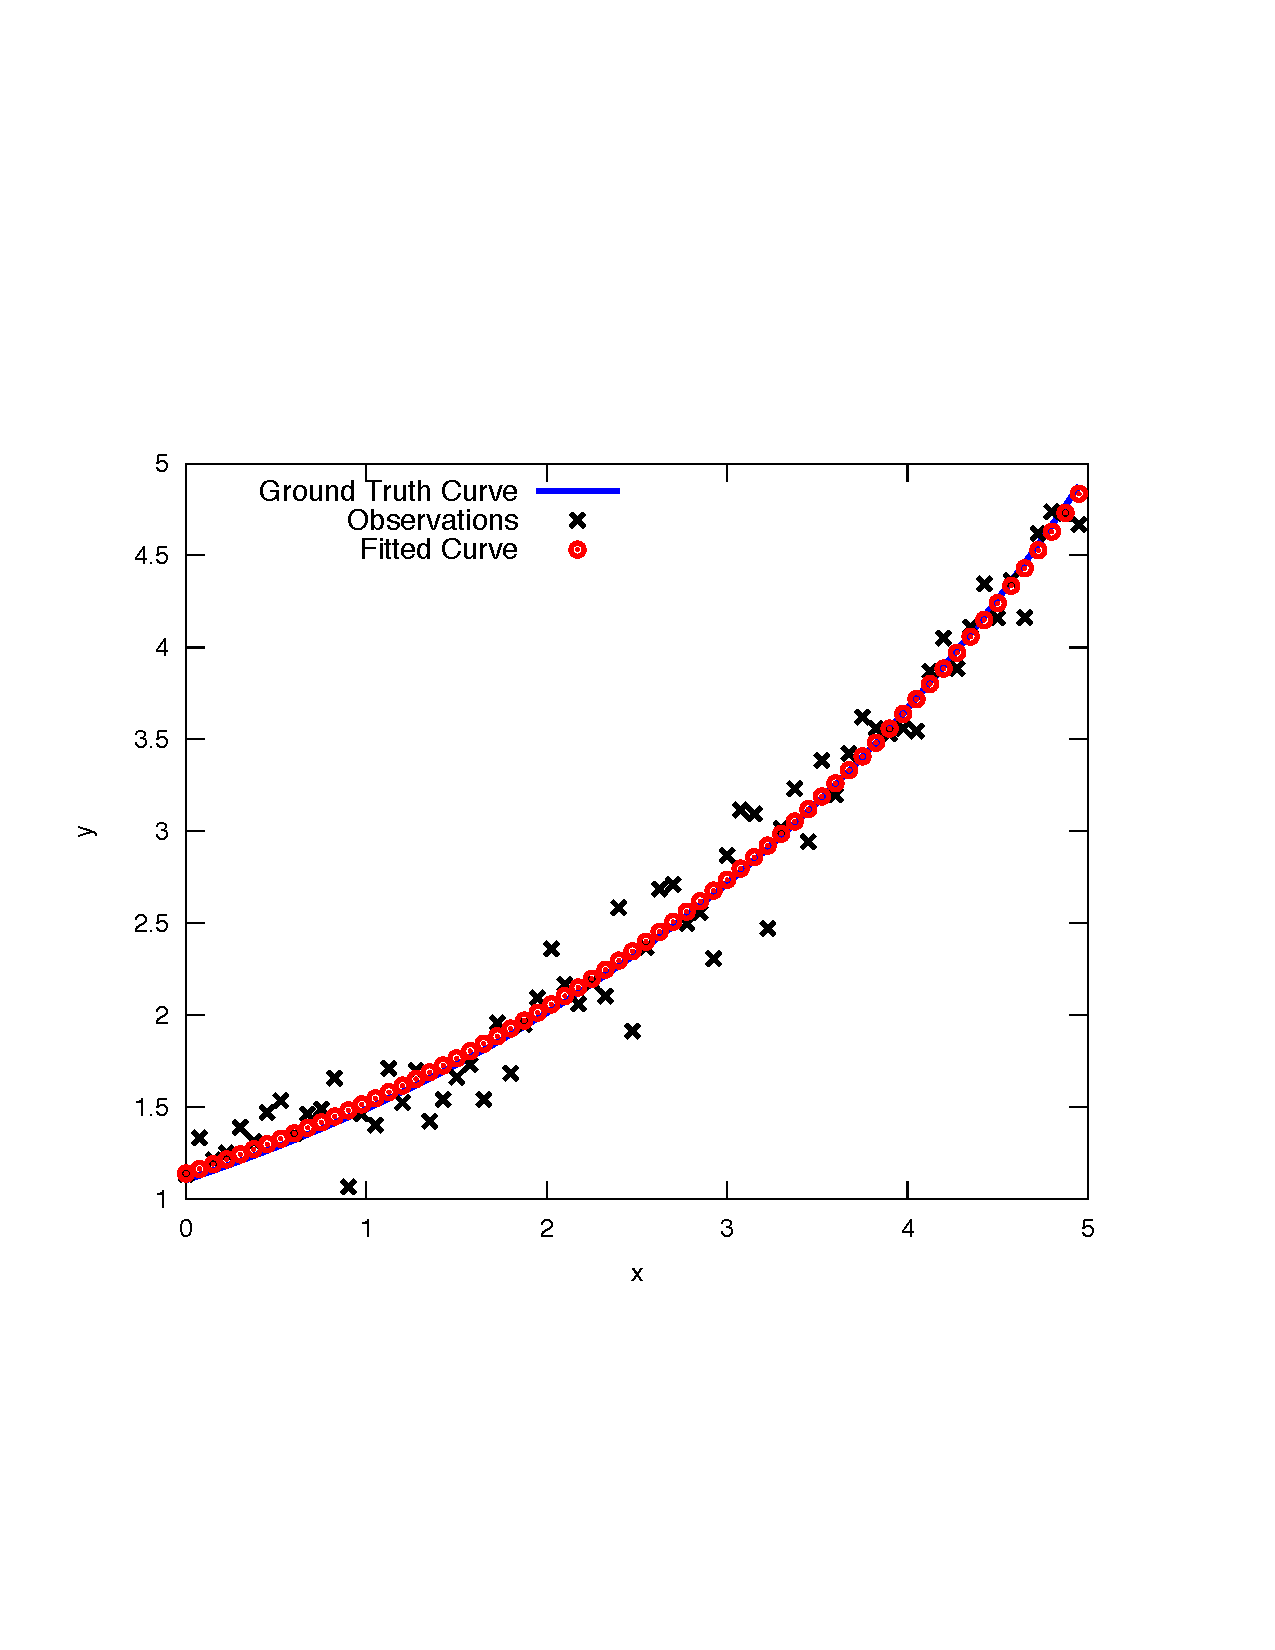
\includegraphics[width=\textwidth]{fit.pdf}
	\caption{Least squares data fitting to the curve $y = e^{0.3x + 0.1}$. Observations were generated by sampling this curve uniformly in the interval $x=(0,5)$ and adding Gaussian noise with $\sigma = 0.2$.\label{fig:exponential}}
\end{center}
\end{figure}

Starting from parameter values $m = 0, c=0$ with an initial objective function value of $121.173$ Ceres finds a solution $m= 0.291861, c = 0.131439$ with an objective function value of $1.05675$. These values are a a bit different than the parameters of the original model $m=0.3, c= 0.1$, but this is expected. When reconstructing a curve from noisy data, we expect to see such deviations. Indeed, if you were to evaluate the objective function for $m=0.3, c=0.1$, the fit is worse with an objective function value of 1.082425. Figure~\ref{fig:exponential} illustrates the fit.

%!TEX root = ceres.tex
\chapter{Bundle Adjustment}
\label{chapter:tutorial:bundleadjustment}
One of the main reasons for writing Ceres was our need to solve large scale bundle adjustment problems~\cite{hartley-zisserman-book-2004,triggs-etal-1999}.

Given a set of measured image feature locations and correspondences, the goal of bundle adjustment is to find 3D point positions and camera parameters that minimize the reprojection error. This optimization problem is usually formulated as a non-linear least squares problem, where the error is the squared $L_2$ norm of the difference between the observed feature location and the projection of the corresponding 3D point on the image plane of the camera. Ceres has extensive support for solving bundle adjustment problems. 

Let us consider the solution of a problem from the BAL~\cite{Agarwal10bal} dataset~\footnote{The code for this example can be found in \texttt{examples/simple\_bundle\_adjuster.cc}.}. 

The first step as usual is to define a templated functor that computes the reprojection error/residual. The structure of the functor is similar to the \texttt{ExponentialResidual}, in that there is an instance of this object responsible for each image observation.


Each residual in a BAL problem depends on a three dimensional point and a nine parameter
camera. The nine parameters defining the camera can are: Three for rotation as a Rodriquez axis-angle vector, three for translation, one for focal length and two for radial distortion.  The details of this camera model can be found on Noah
Snavely's Bundler
homepage~\footnote{\url{http://phototour.cs.washington.edu/bundler/}}
and the BAL
homepage~\footnote{\url{http://grail.cs.washington.edu/projects/bal/}}.


%\begin{listing}[ht]
\clearpage
\begin{minted}[mathescape]{c++}
struct SnavelyReprojectionError {
  SnavelyReprojectionError(double observed_x, double observed_y)
      : observed_x(observed_x), observed_y(observed_y) {}
  template <typename T>
  bool operator()(const T* const camera,
                  const T* const point,
                  T* residuals) const {
    // camera[0,1,2] are the angle-axis rotation.
    T p[3];
    ceres::AngleAxisRotatePoint(camera, point, p);
    // camera[3,4,5] are the translation.
    p[0] += camera[3]; p[1] += camera[4]; p[2] += camera[5];

    // Compute the center of distortion. The sign change comes from
    // the camera model that Noah Snavely's Bundler assumes, whereby
    // the camera coordinate system has a negative z axis.
    const T& focal = camera[6];
    T xp = - focal * p[0] / p[2];
    T yp = - focal * p[1] / p[2];

    // Apply second and fourth order radial distortion.
    const T& l1 = camera[7];
    const T& l2 = camera[8];
    T r2 = xp*xp + yp*yp;
    T distortion = T(1.0) + r2  * (l1 + l2  * r2);

    // Compute final projected point position.
    T predicted_x = distortion * xp;
    T predicted_y = distortion * yp;

    // The error is the difference between the predicted and observed position.
    residuals[0] = predicted_x - T(observed_x);
    residuals[1] = predicted_y - T(observed_y);
    return true;
  }
  double observed_x;
  double observed_y;
};
\end{minted}

Note that unlike the
examples before this is a non-trivial function and computing its
analytic Jacobian is a bit of a pain. Automatic differentiation makes
our life very simple here. The function \texttt{AngleAxisRotatePoint} and other functions for manipulating rotations can be found in \texttt{include/ceres/rotation.h}.  

Given this functor, the bundle adjustment problem can be constructed as follows:
\begin{minted}{c++}
// Create residuals for each observation in the bundle adjustment problem. The
// parameters for cameras and points are added automatically.
ceres::Problem problem;
for (int i = 0; i < bal_problem.num_observations(); ++i) {
  // Each Residual block takes a point and a camera as input and outputs a 2
  // dimensional residual. Internally, the cost function stores the observed
  // image location and compares the reprojection against the observation.
  ceres::CostFunction* cost_function =
      new ceres::AutoDiffCostFunction<SnavelyReprojectionError, 2, 9, 3>(
          new SnavelyReprojectionError(
              bal_problem.observations()[2 * i + 0],
              bal_problem.observations()[2 * i + 1]));
  problem.AddResidualBlock(cost_function,
                           NULL /* squared loss */,
                           bal_problem.mutable_camera_for_observation(i),
                           bal_problem.mutable_point_for_observation(i));
}
\end{minted}
Again note that that the problem construction for bundle adjustment is very similar to the curve fitting example.

One way to solve this problem is to set \texttt{Solver::Options::linear\_solver\_type} to \texttt{SPARSE\_NORMAL\_CHOLESKY} and call \texttt{Solve}. And while this is a reasonable thing to do, bundle adjustment problems have a special sparsity structure that can be exploited to solve them much more efficiently. Ceres provides three specialized solvers (collectively known as Schur based solvers) for this task. The example code uses the simplest of them \texttt{DENSE\_SCHUR}. 
\begin{minted}{c++}
ceres::Solver::Options options;
options.linear_solver_type = ceres::DENSE_SCHUR;
options.ordering_type = ceres::SCHUR;
options.minimizer_progress_to_stdout = true;
ceres::Solver::Summary summary;
ceres::Solve(options, &problem, &summary);
std::cout << summary.FullReport() << "\n";
\end{minted}

For a more sophisticated bundle adjustment example which demonstrates the use of Ceres' more advanced features including its  various linear solvers, robust loss functions and local parameterizations see \texttt{examples/bundle\_adjuster.cc}.

%% Reference
\part{Reference}
\label{part:reference}
%!TEX root = ceres-solver.tex
\chapter{Overview}
\label{chapter:overview}
Ceres solves robustified non-linear least squares problems of the form 
\begin{equation}
\frac{1}{2}\sum_{i=1} \rho_i\left(\left\|f_i\left(x_{i_1},\hdots,x_{i_k}\right)\right\|^2\right).
\label{eq:ceresproblem}
\end{equation}
Where $f_i(\cdot)$ is a  cost function that depends on the parameter blocks $\left[x_{i_1}, \hdots , x_{i_k}\right]$ and  $\rho_i$ is a loss function. In most optimization problems small groups of scalars occur together. For example the three components of a translation vector and the four components of the quaternion that define the pose of a camera. We refer to such a group of small scalars as a Parameter Block. Of course a parameter block can just have a single parameter. 
The term $ \rho_i\left(\left\|f_i\left(x_{i_1},\hdots,x_{i_k}\right)\right\|^2\right)$ is known as a Residual Block. A Ceres problem is a collection of residual blocks, each of which depends on a subset of the parameter blocks.

Solving problems using Ceres consists of two steps.
\begin{enumerate}
\item{Modeling} Define parameter blocks and  residual blocks and build a \texttt{Problem} object containing them.
\item{Solving} Configure and run the solver.
\end{enumerate}

These two steps are mostly independent of each other. This is by design. Modeling the optimization problem should not depend on how the solver and the user should be able to switch between various solver settings and strategies without changing the way the problem is modeled. In the next two chapters we will consider each of these steps in detail.
%!TEX root = ceres-solver.tex
\chapter{Modeling}
\label{chapter:api}
\section{\texttt{CostFunction}}
Given parameter blocks $\left[x_{i_1}, \hdots , x_{i_k}\right]$, a \texttt{CostFunction} is responsible for computing
a vector of residuals and if asked a vector of Jacobian matrices, i.e., given $\left[x_{i_1}, \hdots , x_{i_k}\right]$, compute the vector $f_i\left(x_{i_1},\hdots,x_{k_i}\right)$ and the matrices
\begin{equation}
J_{ij} = \frac{\partial}{\partial x_{i_j}}f_i\left(x_{i_1},\hdots,x_{k_i}\right),\quad \forall j = i_1,\hdots, i_k
\end{equation}
\begin{minted}{c++}
class CostFunction {
 public:
  virtual bool Evaluate(double const* const* parameters,
                        double* residuals,
                        double** jacobians) = 0;
  const vector<int16>& parameter_block_sizes();
  int num_residuals() const;

 protected:
  vector<int16>* mutable_parameter_block_sizes();
  void set_num_residuals(int num_residuals);
};
\end{minted}

The signature of the function (number and sizes of input parameter blocks and number of outputs)
is stored in \texttt{parameter\_block\_sizes\_} and \texttt{num\_residuals\_} respectively. User
code inheriting from this class is expected to set these two members with the
corresponding accessors. This information will be verified by the Problem
when added with \texttt{Problem::AddResidualBlock}.

The most important method here is \texttt{Evaluate}. It implements the residual and Jacobian computation.

\texttt{parameters}  is an array of pointers to arrays containing the various parameter blocks. parameters has the same number of elements as parameter\_block\_sizes\_.  Parameter blocks are in the same order as parameter\_block\_sizes\_.


\texttt{residuals} is an array of size \texttt{num\_residuals\_}.


\texttt{jacobians} is an array of size \texttt{parameter\_block\_sizes\_} containing pointers to storage for Jacobian matrices corresponding to each parameter block. The Jacobian matrices are in the same order as \texttt{parameter\_block\_sizes\_}. \texttt{jacobians[i]} is an array that contains \texttt{num\_residuals\_} $\times$ \texttt{parameter\_block\_sizes\_[i]} elements. Each Jacobian matrix is stored in row-major order, i.e.,

\begin{equation}
\texttt{jacobians[i][r * parameter\_block\_size\_[i] + c]} =
%\frac{\partial}{\partial x_{ic}}  f_{r}\left(x_{1},\hdots, x_{k}\right)
\frac{\partial \texttt{residual[r]}}{\partial \texttt{parameters[i][c]}}
\end{equation}

If \texttt{jacobians} is \texttt{NULL}, then no derivatives are returned; this is the case when computing cost only. If \texttt{jacobians[i]} is \texttt{NULL}, then the Jacobian matrix corresponding to the $i^{\textrm{th}}$ parameter block must not be returned, this is the case when the a parameter block is marked constant.

\section{\texttt{SizedCostFunction}}
If the size of the parameter blocks and the size of the residual vector is known at compile time (this is the common case), Ceres provides \texttt{SizedCostFunction}, where these values can be specified as template parameters.
\begin{minted}{c++}
template<int kNumResiduals,
         int N0 = 0, int N1 = 0, int N2 = 0, int N3 = 0, int N4 = 0, int N5 = 0>
class SizedCostFunction : public CostFunction {
 public:
  virtual bool Evaluate(double const* const* parameters,
                        double* residuals,
                        double** jacobians) = 0;
};
\end{minted}
In this case the user only needs to implement the \texttt{Evaluate} method.

\section{\texttt{AutoDiffCostFunction}}
But even defining the \texttt{SizedCostFunction} can be a tedious affair if complicated derivative computations are involved. To this end Ceres provides automatic differentiation.

To get an auto differentiated cost function, you must define a class with a
 templated \texttt{operator()} (a functor) that computes the cost function in terms of
 the template parameter \texttt{T}. The autodiff framework substitutes appropriate
 \texttt{Jet} objects for T in order to compute the derivative when necessary, but
 this is hidden, and you should write the function as if T were a scalar type
 (e.g. a double-precision floating point number).

 The function must write the computed value in the last argument (the only
 non-\texttt{const} one) and return true to indicate success.

 For example, consider a scalar error $e = k - x^\top y$, where both $x$ and $y$ are
 two-dimensional vector parameters  and $k$ is a constant. The form of this error, which is the
 difference between a constant and an expression, is a common pattern in least
 squares problems. For example, the value $x^\top y$ might be the model expectation
 for a series of measurements, where there is an instance of the cost function
 for each measurement $k$.

 The actual cost added to the total problem is $e^2$, or $(k - x^\top y)^2$; however,
 the squaring is implicitly done by the optimization framework.

 To write an auto-differentiable cost function for the above model, first
 define the object
\begin{minted}{c++}
class MyScalarCostFunction {
  MyScalarCostFunction(double k): k_(k) {}
  template <typename T>
  bool operator()(const T* const x , const T* const y, T* e) const {
    e[0] = T(k_) - x[0] * y[0] + x[1] * y[1]
     return true;
  }

 private:
  double k_;
};
\end{minted}

Note that in the declaration of \texttt{operator()} the input parameters \texttt{x} and \texttt{y} come
 first, and are passed as const pointers to arrays of \texttt{T}. If there were three
 input parameters, then the third input parameter would come after \texttt{y}. The
 output is always the last parameter, and is also a pointer to an array. In
 the example above, \texttt{e} is a scalar, so only \texttt{e[0]} is set.

 Then given this class definition, the auto differentiated cost function for
 it can be constructed as follows.

\begin{minted}{c++}
CostFunction* cost_function
    = new AutoDiffCostFunction<MyScalarCostFunction, 1, 2, 2>(
        new MyScalarCostFunction(1.0));              ^  ^  ^
                                                     |  |  |
                         Dimension of residual ------+  |  |
                         Dimension of x ----------------+  |
                         Dimension of y -------------------+
\end{minted}

In this example, there is usually an instance for each measurement of k.

In the instantiation above, the template parameters following
 \texttt{MyScalarCostFunction}, \texttt{<1, 2, 2>} describe the functor as computing a
 1-dimensional output from two arguments, both 2-dimensional.

 The framework can currently accommodate cost functions of up to 6 independent
 variables, and there is no limit on the dimensionality of each of them.

 \textbf{WARNING 1} Since the functor will get instantiated with different types for
 \texttt{T}, you must convert from other numeric types to \texttt{T} before mixing
 computations with other variables of type \texttt{T}. In the example above, this is
 seen where instead of using \texttt{k\_} directly, \texttt{k\_} is wrapped with \texttt{T(k\_)}.

 \textbf{WARNING 2} A common beginner's error when first using \texttt{AutoDiffCostFunction} is to get the sizing wrong. In particular, there is a tendency to
 set the template parameters to (dimension of residual, number of parameters)
 instead of passing a dimension parameter for {\em every parameter block}. In the
 example above, that would be \texttt{<MyScalarCostFunction, 1, 2>}, which is missing
 the 2 as the last template argument.

\subsection{Theory \& Implementation}
TBD

\section{\texttt{NumericDiffCostFunction}}
To get a numerically differentiated cost function, define a subclass of
\texttt{CostFunction} such that the \texttt{Evaluate} function ignores the jacobian
parameter. The numeric differentiation wrapper will fill in the jacobians array
 if necessary by repeatedly calling the \texttt{Evaluate} method with
small changes to the appropriate parameters, and computing the slope. For
performance, the numeric differentiation wrapper class is templated on the
concrete cost function, even though it could be implemented only in terms of
the virtual \texttt{CostFunction} interface.
\begin{minted}{c++}
template <typename CostFunctionNoJacobian,
          NumericDiffMethod method = CENTRAL, int M = 0,
          int N0 = 0, int N1 = 0, int N2 = 0, int N3 = 0, int N4 = 0, int N5 = 0>
class NumericDiffCostFunction
    : public SizedCostFunction<M, N0, N1, N2, N3, N4, N5> {
};
\end{minted}

The numerically differentiated version of a cost function for a cost function
can be constructed as follows:
\begin{minted}{c++}
CostFunction* cost_function
    = new NumericDiffCostFunction<MyCostFunction, CENTRAL, 1, 4, 8>(
        new MyCostFunction(...), TAKE_OWNERSHIP);
\end{minted}
where \texttt{MyCostFunction} has 1 residual and 2 parameter blocks with sizes 4 and 8
respectively. Look at the tests for a more detailed example.

The central difference method is considerably more accurate at the cost of
twice as many function evaluations than forward difference. Consider using
central differences begin with, and only after that works, trying forward
difference to improve performance.

\section{\texttt{LossFunction}}
 For least squares problems where the minimization may encounter
 input terms that contain outliers, that is, completely bogus
 measurements, it is important to use a loss function that reduces
 their influence.

 Consider a structure from motion problem. The unknowns are 3D
 points and camera parameters, and the measurements are image
 coordinates describing the expected reprojected position for a
 point in a camera. For example, we want to model the geometry of a
 street scene with fire hydrants and cars, observed by a moving
 camera with unknown parameters, and the only 3D points we care
 about are the pointy tippy-tops of the fire hydrants. Our magic
 image processing algorithm, which is responsible for producing the
 measurements that are input to Ceres, has found and matched all
 such tippy-tops in all image frames, except that in one of the
 frame it mistook a car's headlight for a hydrant. If we didn't do
 anything special  the
 residual for the erroneous measurement will result in the
 entire solution getting pulled away from the optimum to reduce
 the large error that would otherwise be attributed to the wrong
 measurement.

 Using a robust loss function, the cost for large residuals is
 reduced. In the example above, this leads to outlier terms getting
 down-weighted so they do not overly influence the final solution.

\begin{minted}{c++}
class LossFunction {
 public:
  virtual void Evaluate(double s, double out[3]) const = 0;
};
\end{minted}

The key method is \texttt{Evaluate}, which given a non-negative scalar \texttt{s}, computes
\begin{align}
	\texttt{out} = \begin{bmatrix}\rho(s), & \rho'(s), & \rho''(s)\end{bmatrix}
\end{align}

Here the convention is that the contribution of a term to the cost function is given by $\frac{1}{2}\rho(s)$,  where $s = \|f_i\|^2$. Calling the method with a negative value of $s$ is an error and the implementations are not required to handle that case.

Most sane choices of $\rho$ satisfy:
\begin{align}
   \rho(0) &= 0\\
   \rho'(0) &= 1\\
   \rho'(s) &< 1 \text{ in the outlier region}\\
   \rho''(s) &< 0 \text{ in the outlier region}
\end{align}
so that they mimic the squared cost for small residuals.

\subsection{Scaling}
Given one robustifier $\rho(s)$
 one can change the length scale at which robustification takes
 place, by adding a scale factor $a > 0$ which gives us $\rho(s,a) = a^2 \rho(s / a^2)$ and the first and second derivatives as $\rho'(s / a^2)$ and   $(1 / a^2) \rho''(s / a^2)$ respectively.


\begin{figure}[hbt]
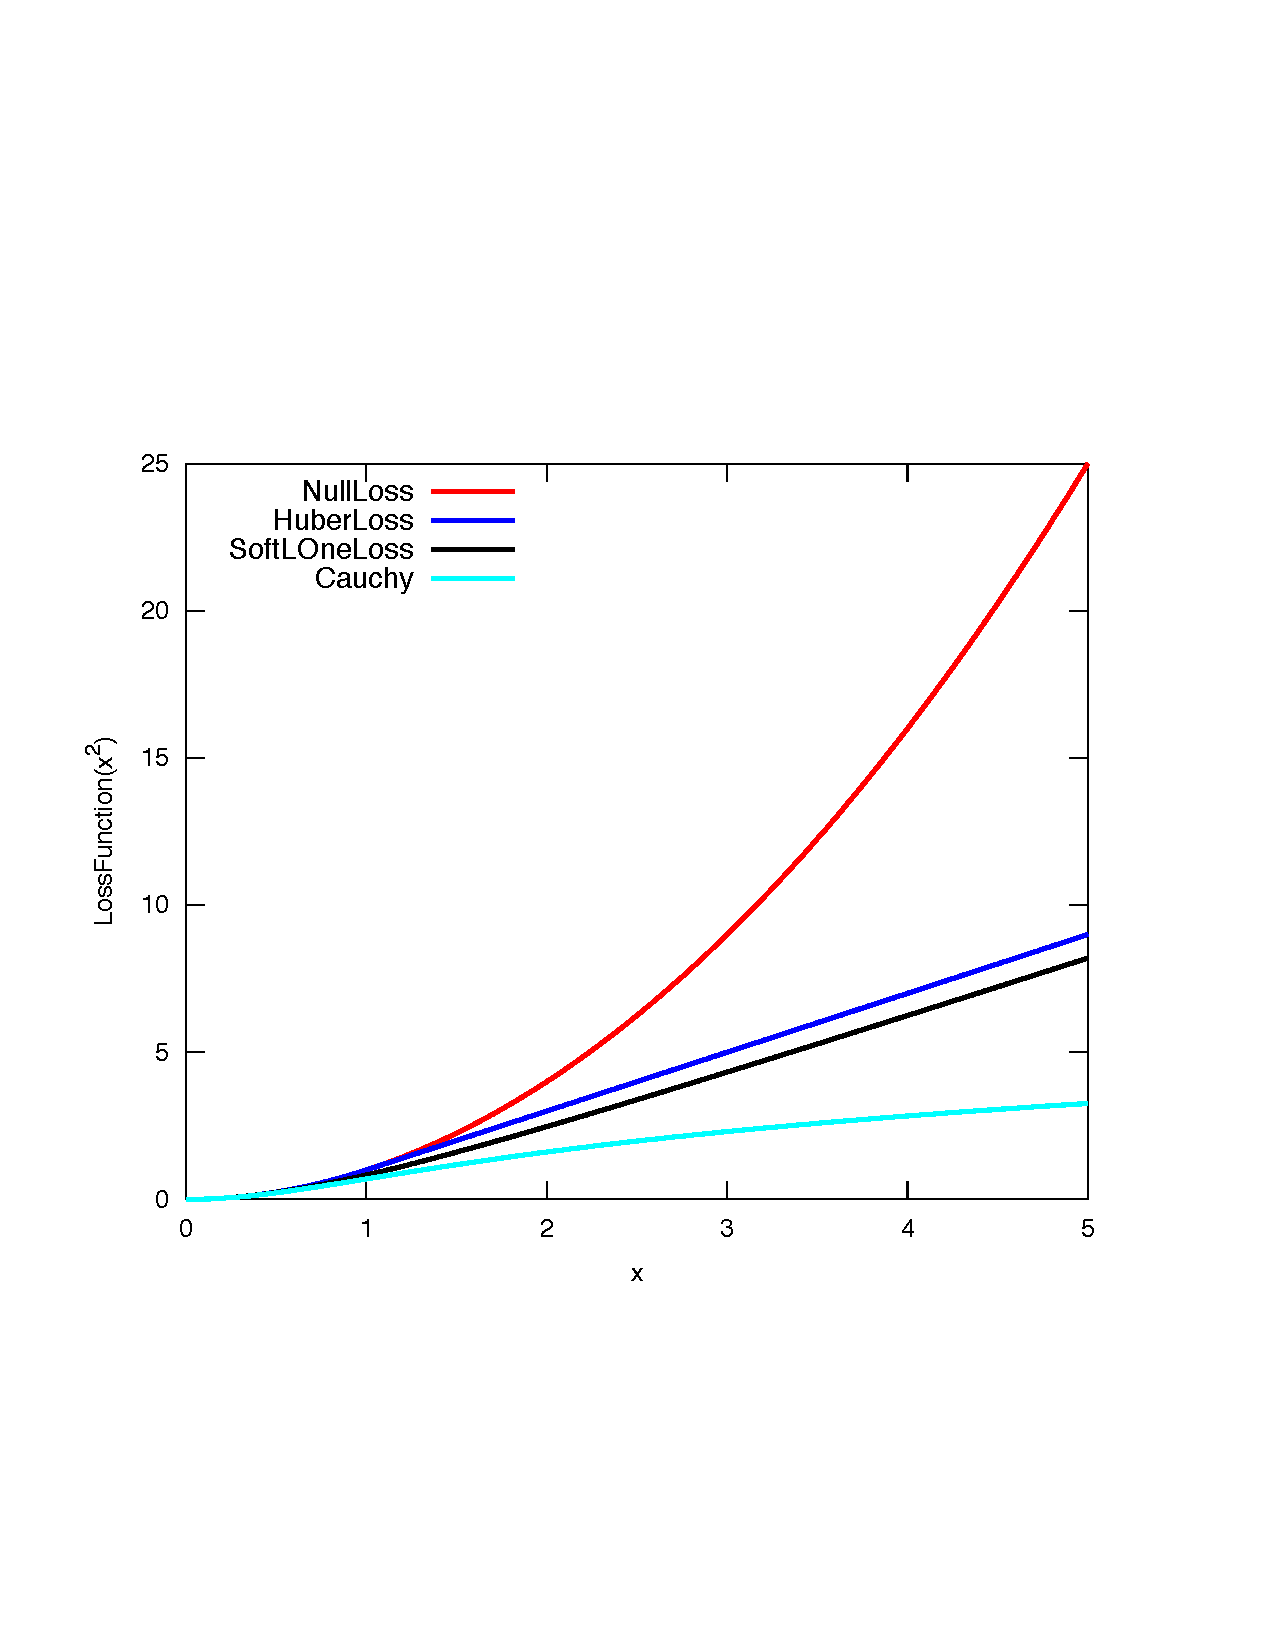
\includegraphics[width=\textwidth]{loss.pdf}
\caption{Shape of the various common loss functions.}
\label{fig:loss}
\end{figure}


The reason for the appearance of squaring is that $a$ is in the units of the residual vector norm whereas $s$ is a squared norm. For applications it is more convenient to specify $a$ than
its square.

Here are some common loss functions implemented in Ceres. For simplicity we described their unscaled versions. Figure~\ref{fig:loss} illustrates their shape graphically.

\begin{align}
		\rho(s)&=s \tag{\texttt{NullLoss}}\\
		\rho(s) &= \begin{cases}
		       s & s \le 1\\
		       2 \sqrt{s} - 1 & s > 1
	           \end{cases} \tag{\texttt{HuberLoss}}\\
		\rho(s) &= 2 (\sqrt{1+s} - 1) \tag{\texttt{SoftLOneLoss}}\\
		\rho(s) &= \log(1 + s) \tag{\texttt{CauchyLoss}}
\end{align}

Ceres includes a number of other loss functions, the descriptions and
documentation for which can be found in \texttt{loss\_function.h}.
\subsection{Theory \& Implementation}
TBD

\section{\texttt{LocalParameterization}}
Sometimes the parameters $x$ can overparameterize a problem. In
that case it is desirable to choose a parameterization to remove
the null directions of the cost. More generally, if $x$ lies on a
manifold of a smaller dimension than the ambient space that it is
embedded in, then it is numerically and computationally more
effective to optimize it using a parameterization that lives in
the tangent space of that manifold at each point.

For example, a sphere in three dimensions is a two dimensional
manifold, embedded in a three dimensional space. At each point on
the sphere, the plane tangent to it defines a two dimensional
tangent space. For a cost function defined on this sphere, given a
point $x$, moving in the direction normal to the sphere at that
point is not useful. Thus a better way to parameterize a point on
a sphere is to optimize over two dimensional vector $\Delta x$ in the
tangent space at the point on the sphere point and then "move" to
the point $x + \Delta x$, where the move operation involves projecting
back onto the sphere. Doing so removes a redundant dimension from
the optimization, making it numerically more robust and efficient.

More generally we can define a function
\begin{equation}
  x' = \boxplus(x, \Delta x),
\end{equation}
where $x'$ has the same size as $x$, and $\Delta x$ is of size less
than or equal to $x$. The function $\boxplus$, generalizes the
definition of vector addition. Thus it satisfies the identity
\begin{equation}
  \boxplus(x, 0) = x,\quad \forall x.
\end{equation}

Instances of \texttt{LocalParameterization} implement the $\boxplus$ operation and its derivative with respect to $\Delta x$ at $\Delta x = 0$.

\begin{minted}{c++}
class LocalParameterization {
 public:
  virtual ~LocalParameterization() {}
  virtual bool Plus(const double* x,
                    const double* delta,
                    double* x_plus_delta) const = 0;
  virtual bool ComputeJacobian(const double* x, double* jacobian) const = 0;
  virtual int GlobalSize() const = 0;
  virtual int LocalSize() const = 0;
};
\end{minted}

\texttt{GlobalSize} is the dimension of the ambient space in which the parameter block $x$ lives. \texttt{LocalSize} is the size of the tangent space that $\Delta x$ lives in. \texttt{Plus} implements $\boxplus(x,\Delta x)$ and $\texttt{ComputeJacobian}$ computes the Jacobian matrix
\begin{equation}
	J = \left . \frac{\partial }{\partial \Delta x} \boxplus(x,\Delta x)\right|_{\Delta x = 0}
\end{equation}
in row major form.

A trivial version of $\boxplus$ is when delta is of the same size as $x$
and

\begin{equation}
  \boxplus(x, \Delta x) = x + \Delta x
\end{equation}

A more interesting case if $x$ is a two dimensional vector, and the
user wishes to hold the first coordinate constant. Then, $\Delta x$ is a
scalar and $\boxplus$ is defined as

\begin{equation}
  \boxplus(x, \Delta x) = x + \left[ \begin{array}{c} 0 \\ 1
                                  \end{array} \right]        \Delta x
\end{equation}

\texttt{SubsetParameterization} generalizes this construction to hold any part of a parameter block constant.


Another example that occurs commonly in Structure from Motion problems
is when camera rotations are parameterized using a quaternion. There,
it is useful only to make updates orthogonal to that 4-vector defining
the quaternion. One way to do this is to let $\Delta x$ be a 3
dimensional vector and define $\boxplus$ to be

\begin{equation}
  \boxplus(x, \Delta x) =
\left[
\cos(|\Delta x|), \frac{\sin\left(|\Delta x|\right)}{|\Delta x|} \Delta x
\right] * x
\label{eq:quaternion}
\end{equation}
The multiplication between the two 4-vectors on the right hand
side is the standard quaternion product. \texttt{QuaternionParameterization} is an implementation of~\eqref{eq:quaternion}.

\clearpage

\section{\texttt{Problem}}
\begin{minted}{c++}
class Problem {
 public:
  struct Options {
    Options();
    Ownership cost_function_ownership;
    Ownership loss_function_ownership;
    Ownership local_parameterization_ownership;
  };

  Problem();
  explicit Problem(const Options& options);
  ~Problem();

  ResidualBlockId AddResidualBlock(CostFunction* cost_function,
                                   LossFunction* loss_function,
                                   const vector<double*>& parameter_blocks);

  void AddParameterBlock(double* values, int size);
  void AddParameterBlock(double* values,
                         int size,
                         LocalParameterization* local_parameterization);

  void SetParameterBlockConstant(double* values);
  void SetParameterBlockVariable(double* values);
  void SetParameterization(double* values,
                           LocalParameterization* local_parameterization);

  int NumParameterBlocks() const;
  int NumParameters() const;
  int NumResidualBlocks() const;
  int NumResiduals() const;
};
\end{minted}

The \texttt{Problem} objects holds the robustified non-linear least squares problem~\eqref{eq:ceresproblem}. To create a least squares problem, use the \texttt{Problem::AddResidualBlock} and \texttt{Problem::AddParameterBlock} methods.

For example a problem containing 3 parameter blocks of sizes 3, 4 and 5
respectively and two residual blocks  of size 2 and 6:

\begin{minted}{c++}
double x1[] = { 1.0, 2.0, 3.0 };
double x2[] = { 1.0, 2.0, 3.0, 5.0 };
double x3[] = { 1.0, 2.0, 3.0, 6.0, 7.0 };

Problem problem;
problem.AddResidualBlock(new MyUnaryCostFunction(...), x1);
problem.AddResidualBlock(new MyBinaryCostFunction(...), x2, x3);
\end{minted}


\texttt{AddResidualBlock} as the name implies, adds a residual block to the problem. It adds a cost function, an optional loss function, and connects the cost function to a set of parameter blocks.

The cost
   function carries with it information about the sizes of the
   parameter blocks it expects. The function checks that these match
   the sizes of the parameter blocks listed in \texttt{parameter\_blocks}. The
   program aborts if a mismatch is detected. \texttt{loss\_function} can be
   \texttt{NULL}, in which case the cost of the term is just the squared norm
   of the residuals.

  The user has the option of explicitly adding the parameter blocks
  using \texttt{AddParameterBlock}. This causes additional correctness
  checking; however, \texttt{AddResidualBlock} implicitly adds the parameter
   blocks if they are not present, so calling \texttt{AddParameterBlock}
   explicitly is not required.


   \texttt{Problem} by default takes ownership of the
  \texttt{cost\_function} and \texttt{loss\_function pointers}. These objects remain
   live for the life of the \texttt{Problem} object. If the user wishes to
  keep control over the destruction of these objects, then they can
  do this by setting the corresponding enums in the \texttt{Options} struct.


  Note that even though the Problem takes ownership of \texttt{cost\_function}
  and \texttt{loss\_function}, it does not preclude the user from re-using
  them in another residual block. The destructor takes care to call
  delete on each \texttt{cost\_function} or \texttt{loss\_function} pointer only once,
  regardless of how many residual blocks refer to them.

\texttt{AddParameterBlock} explicitly adds a parameter block to the \texttt{Problem}. Optionally it allows the user to associate a LocalParameterization object with the parameter block too. Repeated calls with the same arguments are ignored. Repeated
calls with the same double pointer but a different size results in undefined behaviour.

You can set any parameter block to be constant using

\texttt{Problem::SetParameterBlockConstant}

and undo this using

\texttt{Problem::SetParameterBlockVariable}.

In fact you can set any number of parameter blocks to be constant, and Ceres is smart enough to figure out what part of the problem you have constructed depends on the parameter blocks that are free to change and only spends time solving it. So for example if you constructed a problem with a million parameter blocks and 2 million residual blocks, but then set all but one parameter blocks to be constant and say only 10 residual blocks depend on this one non-constant parameter block. Then the computational effort Ceres spends in solving this problem will be the same if you had defined a problem with one parameter block and 10 residual blocks.

  \texttt{Problem} by default takes ownership of the
  \texttt{cost\_function}, \texttt{loss\_function} and \\ \texttt{local\_parameterization} pointers. These objects remain
   live for the life of the \texttt{Problem} object. If the user wishes to
  keep control over the destruction of these objects, then they can
  do this by setting the corresponding enums in the \texttt{Options} struct. Even though \texttt{Problem} takes ownership of these pointers,  it does not preclude the user from re-using them in another residual or parameter block. The destructor takes care to call
  delete on each  pointer only once.

%!TEX root = ceres-solver.tex
\chapter{Solving}
Effective use of Ceres requires some familiarity with the basic components of a nonlinear least squares solver, so before we describe how to configure the solver, we will begin by taking a brief look at how some of the core optimization algorithms in Ceres work and the various linear solvers and preconditioners that power it.

\section{Trust Region Methods}
\label{sec:trust-region}
Let $x \in \mathbb{R}^{n}$ be an $n$-dimensional vector of variables, and
$ F(x) = \left[f_1(x),   \hdots,  f_{m}(x) \right]^{\top}$ be a $m$-dimensional function of $x$.  We are interested in solving the following optimization problem~\footnote{At the level of the non-linear solver, the block and residual structure is not relevant, therefore our discussion here is in terms of an optimization problem defined over a state vector of size $n$.},
\begin{equation}
        \arg \min_x \frac{1}{2}\|F(x)\|^2\ .
        \label{eq:nonlinsq}
\end{equation}
Here, the Jacobian $J(x)$ of $F(x)$ is an $m\times n$ matrix, where $J_{ij}(x) = \partial_j f_i(x)$  and the gradient vector $g(x) = \nabla  \frac{1}{2}\|F(x)\|^2 = J(x)^\top F(x)$. Since the efficient global optimization of~\eqref{eq:nonlinsq} for general $F(x)$ is an intractable problem, we will have to settle for finding a local minimum.

The general strategy when solving non-linear optimization problems is to solve a sequence of approximations to the original problem~\cite{nocedal2000numerical}. At each iteration, the approximation is solved to determine a correction $\Delta x$ to the vector $x$. For non-linear least squares, an approximation can be constructed by using the linearization $F(x+\Delta x) \approx F(x) + J(x)\Delta x$, which leads to the following linear least squares  problem:
\begin{equation}
         \min_{\Delta x} \frac{1}{2}\|J(x)\Delta x + F(x)\|^2
        \label{eq:linearapprox}
\end{equation}
Unfortunately, na\"ively solving a sequence of these problems and
updating $x \leftarrow x+ \Delta x$ leads to an algorithm that may not
converge.  To get a convergent algorithm, we need to control the size
of the step $\Delta x$. And this is where the idea of a trust-region
comes in. Algorithm~\ref{alg:trust-region} describes the basic  trust-region loop for non-linear least squares problems.

\begin{algorithm}
\caption{The basic trust-region algorithm.\label{alg:trust-region}}
\begin{algorithmic}
\REQUIRE Initial point $x$ and a trust region radius $\mu$.
\LOOP
\STATE{Solve $\arg \min_{\Delta x} \frac{1}{2}\|J(x)\Delta x + F(x)\|^2$ s.t. $\|D(x)\Delta x\|^2 \le \mu$}
\STATE{$\rho = \frac{\displaystyle \|F(x + \Delta x)\|^2 - \|F(x)\|^2}{\displaystyle \|J(x)\Delta x + F(x)\|^2 - \|F(x)\|^2}$}
\IF {$\rho > \epsilon$}
\STATE{$x = x + \Delta x$}
\ENDIF
\IF {$\rho > \eta_1$}
\STATE{$\rho = 2 * \rho$}
\ELSE
\IF {$\rho < \eta_2$}
\STATE {$\rho = 0.5 * \rho$}
\ENDIF
\ENDIF
\ENDLOOP
\end{algorithmic}
\end{algorithm}

Here, $\mu$ is the trust region radius, $D(x)$ is some matrix used to define a metric on the domain of $F(x)$ and $\rho$ measures the quality of the step $\Delta x$, i.e., how well did the linear model predict the decrease in the value of the non-linear objective. The idea is to increase or decrease the radius of the trust region depending on how well the linearization predicts the behavior of the non-linear objective, which in turn is reflected in the value of $\rho$.

The key computational step in a trust-region algorithm is the solution of the constrained optimization problem
\begin{align}
        \arg\min_{\Delta x}& \frac{1}{2}\|J(x)\Delta x + F(x)\|^2 \\
        \text{such that}&\quad  \|D(x)\Delta x\|^2 \le \mu
\label{eq:trp}
\end{align}

There are a number of different ways of solving this problem, each giving rise to a different concrete trust-region algorithm. Currently Ceres, implements two trust-region algorithms - Levenberg-Marquardt and  Dogleg.

\subsection{Levenberg-Marquardt}
The Levenberg-Marquardt algorithm~\cite{levenberg1944method, marquardt1963algorithm} is the most popular algorithm for solving non-linear least squares problems.  It was also the first trust region algorithm to be developed~\cite{levenberg1944method,marquardt1963algorithm}. Ceres implements an exact step~\cite{madsen2004methods} and an inexact step variant of the Levenberg-Marquardt algorithm~\cite{wright1985inexact,nash1990assessing}.

It can be shown, that the solution to~\eqref{eq:trp} can be obtained by solving an unconstrained optimization of the form
\begin{align}
        \arg\min_{\Delta x}& \frac{1}{2}\|J(x)\Delta x + F(x)\|^2 +\lambda  \|D(x)\Delta x\|^2
\end{align}
Where, $\lambda$ is a Lagrange multiplier that is inverse related to $\mu$. In Ceres, we solve for
\begin{align}
        \arg\min_{\Delta x}& \frac{1}{2}\|J(x)\Delta x + F(x)\|^2 + \frac{1}{\mu} \|D(x)\Delta x\|^2
\label{eq:lsqr}
\end{align}
The matrix $D(x)$ is a non-negative diagonal matrix, typically the square root of the diagonal of the matrix $J(x)^\top J(x)$.

Before going further, let us make some notational simplifications. We will assume that the matrix $\sqrt{\mu} D$ has been concatenated at the bottom of the matrix $J$ and similarly a vector of zeros has been added to the bottom of the vector $f$ and the rest of our discussion will be in terms of $J$ and $f$, \ie the linear least squares problem.
\begin{align}
 \min_{\Delta x} \frac{1}{2} \|J(x)\Delta x + f(x)\|^2 .
 \label{eq:simple}
\end{align}
For all but the smallest problems the solution of~\eqref{eq:simple} in each iteration of the Levenberg-Marquardt algorithm is the dominant computational cost in Ceres. Ceres provides a number of different options for solving~\eqref{eq:simple}. There are two major classes of methods - factorization and iterative.

The factorization methods are based on computing an exact solution of~\eqref{eq:lsqr} using a Cholesky or a QR factorization and lead to an exact step Levenberg-Marquardt algorithm. But it is not clear if an exact solution of~\eqref{eq:lsqr} is necessary at each step of the LM algorithm to solve~\eqref{eq:nonlinsq}. In fact, we have already seen evidence that this may not be the case, as~\eqref{eq:lsqr} is itself a regularized version of~\eqref{eq:linearapprox}. Indeed, it is possible to construct non-linear optimization algorithms in which the linearized problem is solved approximately. These algorithms are known as inexact Newton or truncated Newton methods~\cite{nocedal2000numerical}.

An inexact Newton method requires two ingredients. First, a cheap method for approximately solving systems of linear equations. Typically an iterative linear solver like the Conjugate Gradients method is used for this purpose~\cite{nocedal2000numerical}. Second, a termination rule for the iterative solver. A typical termination rule is of the form
\begin{equation}
        \|H(x) \Delta x + g(x)\| \leq \eta_k \|g(x)\|. \label{eq:inexact}
\end{equation}
Here, $k$ indicates the Levenberg-Marquardt iteration number and $0 < \eta_k <1$ is known as the forcing sequence.  Wright \& Holt \cite{wright1985inexact} prove that a truncated Levenberg-Marquardt algorithm that uses an inexact Newton step based on~\eqref{eq:inexact} converges for any sequence $\eta_k \leq \eta_0 < 1$ and the rate of convergence depends on the choice of the forcing sequence $\eta_k$.

Ceres supports both exact and inexact step solution strategies. When the user chooses a factorization based linear solver, the exact step Levenberg-Marquardt algorithm is used. When the user chooses an iterative linear solver, the inexact step Levenberg-Marquardt algorithm is used.

\subsection{Dogleg}
\label{sec:dogleg}
Another strategy for solving the trust region problem~\eqref{eq:trp} was introduced by M. J. D. Powell. The key idea there is to compute two vectors
\begin{align}
        \Delta x^{\text{Gauss-Newton}} &= \arg \min_{\Delta x}\frac{1}{2} \|J(x)\Delta x + f(x)\|^2.\\
        \Delta x^{\text{Cauchy}} &= -\frac{\|g(x)\|^2}{\|J(x)g(x)\|^2}g(x).
\end{align}
Note that the vector $\Delta x^{\text{Gauss-Newton}}$ is the solution
to~\eqref{eq:linearapprox} and $\Delta x^{\text{Cauchy}}$ is the
vector that minimizes the linear approximation if we restrict
ourselves to moving along the direction of the gradient. Dogleg methods finds a vector $\Delta x$ defined by $\Delta
x^{\text{Gauss-Newton}}$ and $\Delta x^{\text{Cauchy}}$ that solves
the trust region problem. Ceres supports two
variants.

\texttt{TRADITIONAL\_DOGLEG} as described by Powell,
constructs two line segments using the Gauss-Newton and Cauchy vectors
and finds the point farthest along this line shaped like a dogleg
(hence the name) that is contained in the
trust-region. For more details on the exact reasoning and computations, please see Madsen et al~\cite{madsen2004methods}.

 \texttt{SUBSPACE\_DOGLEG} is a more sophisticated method
that considers the entire two dimensional subspace spanned by these
two vectors and finds the point that minimizes the trust region
problem in this subspace\cite{byrd1988approximate}.

The key advantage of the Dogleg over Levenberg Marquardt is that if the step computation for a particular choice of $\mu$ does not result in sufficient decrease in the value of the objective function, Levenberg-Marquardt solves the linear approximation from scratch with a smaller value of $\mu$. Dogleg on the other hand, only needs to compute the interpolation between the Gauss-Newton and the Cauchy vectors, as neither of them depend on the value of $\mu$.

The Dogleg method can only be used with the exact factorization based linear solvers.

\subsection{Inner Iterations}
\label{sec:inner}
Some non-linear least squares problems have additional structure in
the way the parameter blocks interact that it is beneficial to modify
the way the trust region step is computed. e.g., consider the
following regression problem

\begin{equation}
  y = a_1 e^{b_1 x} + a_2 e^{b_3 x^2 + c_1}
\end{equation}

Given a set of pairs $\{(x_i, y_i)\}$, the user wishes to estimate
$a_1, a_2, b_1, b_2$, and $c_1$.

Notice that the expression on the left is linear in $a_1$ and $a_2$,
and given any value for $b_1$, $b_2$ and $c_1$, it is possible to use
linear regression to estimate the optimal values of $a_1$ and
$a_2$. It's possible to analytically eliminate the variables
$a_1$ and $a_2$ from the problem entirely. Problems like these are
known as separable least squares problem and the most famous algorithm
for solving them is the Variable Projection algorithm invented by
Golub \& Pereyra~\cite{golub-pereyra-73}.

Similar structure can be found in the matrix factorization with
missing data problem. There the corresponding algorithm is
known as Wiberg's algorithm~\cite{wiberg}.

Ruhe \& Wedin  present an analysis of
various algorithms for solving separable non-linear least
squares problems and refer to {\em Variable Projection} as
Algorithm I in their paper~\cite{ruhe-wedin}.

Implementing Variable Projection is tedious and expensive. Ruhe \&
Wedin present a simpler algorithm with comparable convergence
properties, which they call Algorithm II.  Algorithm II performs an
additional optimization step to estimate $a_1$ and $a_2$ exactly after
computing a successful Newton step.


This idea can be generalized to cases where the residual is not
linear in $a_1$ and $a_2$, i.e.,

\begin{equation}
  y = f_1(a_1, e^{b_1 x}) + f_2(a_2, e^{b_3 x^2 + c_1})
\end{equation}

In this case, we solve for the trust region step for the full problem,
and then use it as the starting point to further optimize just $a_1$
and $a_2$. For the linear case, this amounts to doing a single linear
least squares solve. For non-linear problems, any method for solving
the $a_1$ and $a_2$ optimization problems will do. The only constraint
on $a_1$ and $a_2$ (if they are two different parameter block) is that
they do not co-occur in a residual block.

This idea can be further generalized, by not just optimizing $(a_1,
a_2)$, but decomposing the graph corresponding to the Hessian matrix's
sparsity structure into a collection of non-overlapping independent sets
and optimizing each of them.

Setting \texttt{Solver::Options::use\_inner\_iterations} to true
enables
the use of this non-linear generalization of Ruhe \& Wedin's Algorithm
II.  This version of Ceres has a higher iteration complexity, but also
displays better convergence behavior per iteration.

Setting \texttt{Solver::Options::num\_threads} to the maximum number
possible is highly recommended.

\subsection{Non-monotonic Steps}
\label{sec:non-monotonic}
Note that the basic trust-region algorithm described in
Algorithm~\ref{alg:trust-region} is a descent algorithm  in that they
only accepts a point if it strictly reduces the value of the objective
function.

Relaxing this requirement allows the algorithm to be more
efficient in the long term at the cost of some local increase
in the value of the objective function.

This is because allowing for non-decreasing objective function
values in a princpled manner allows the algorithm to ``jump over
boulders'' as the method is not restricted to move into narrow
valleys while preserving its convergence properties.

Setting \texttt{Solver::Options::use\_nonmonotonic\_steps} to \texttt{true}
enables the non-monotonic trust region algorithm as described by
Conn,  Gould \& Toint in~\cite{conn2000trust}.

Even though the value of the objective function may be larger
than the minimum value encountered over the course of the
optimization, the final parameters returned to the user are the
ones corresponding to the minimum cost over all iterations.

The option to take non-monotonic is available for all trust region
strategies.

\section{\texttt{LinearSolver}}
Recall that in both of the trust-region methods described above, the key computational cost is the solution of a linear least squares problem of the form
\begin{align}
 \min_{\Delta x} \frac{1}{2} \|J(x)\Delta x + f(x)\|^2 .
 \label{eq:simple2}
\end{align}


Let $H(x)= J(x)^\top J(x)$ and $g(x) = -J(x)^\top  f(x)$. For notational convenience let us also drop the dependence on $x$. Then it is easy to see that solving~\eqref{eq:simple2} is equivalent to solving the {\em normal equations}
\begin{align}
H \Delta x  &= g \label{eq:normal}
\end{align}

Ceres provides a number of different options for solving~\eqref{eq:normal}.

\subsection{\texttt{DENSE\_QR}}
For small problems (a couple of hundred parameters and a few thousand residuals) with relatively dense Jacobians, \texttt{DENSE\_QR} is the method of choice~\cite{bjorck1996numerical}. Let $J = QR$ be the QR-decomposition of $J$, where $Q$ is an orthonormal matrix and $R$ is an upper triangular matrix~\cite{trefethen1997numerical}. Then it can be shown that the solution to~\eqref{eq:normal} is given by
\begin{align}
    \Delta x^* = -R^{-1}Q^\top f
\end{align}
Ceres uses \texttt{Eigen}'s dense QR factorization routines.

\subsection{\texttt{DENSE\_NORMAL\_CHOLESKY} \& \texttt{SPARSE\_NORMAL\_CHOLESKY}}
Large non-linear least square problems are usually sparse. In such cases, using a dense QR factorization is inefficient. Let $H = R^\top R$ be the Cholesky factorization of the normal equations, where $R$ is an upper triangular matrix, then the  solution to ~\eqref{eq:normal} is given by
\begin{equation}
    \Delta x^* = R^{-1} R^{-\top} g.
\end{equation}
The observant reader will note that the $R$ in the Cholesky
factorization of $H$ is the same upper triangular matrix $R$ in the QR
factorization of $J$. Since $Q$ is an orthonormal matrix, $J=QR$
implies that $J^\top J = R^\top Q^\top Q R = R^\top R$. There are two variants of Cholesky factorization -- sparse and
dense.

\texttt{DENSE\_NORMAL\_CHOLESKY}  as the name implies performs a dense
Cholesky factorization of the normal equations. Ceres uses
\texttt{Eigen}'s dense LDLT factorization routines.

\texttt{SPARSE\_NORMAL\_CHOLESKY}, as the name implies performs a
sparse Cholesky factorization of the normal equations. This leads to
substantial savings in time and memory for large sparse
problems. Ceres uses the sparse Cholesky factorization routines in  Professor Tim Davis'  \texttt{SuiteSparse} or
\texttt{CXSparse} packages~\cite{chen2006acs}.

\subsection{\texttt{DENSE\_SCHUR} \& \texttt{SPARSE\_SCHUR}}
While it is possible to use \texttt{SPARSE\_NORMAL\_CHOLESKY} to solve bundle adjustment problems, bundle adjustment problem have a special structure, and a more efficient scheme for solving~\eqref{eq:normal} can be constructed.

Suppose that the SfM problem consists of $p$ cameras and $q$ points and the variable vector $x$ has the  block structure $x = [y_{1},\hdots,y_{p},z_{1},\hdots,z_{q}]$. Where, $y$ and $z$ correspond to camera and point parameters, respectively.  Further, let the camera blocks be of size $c$ and the point blocks be of size $s$ (for most problems $c$ =  $6$--$9$ and $s = 3$). Ceres does not impose any constancy requirement on these block sizes, but choosing them to be constant simplifies the exposition.

A key characteristic of the bundle adjustment problem is that there is no term $f_{i}$ that includes two or more point blocks.  This in turn implies that the matrix $H$ is of the form
\begin{equation}
        H =  \left[
                \begin{matrix} B & E\\ E^\top & C
                \end{matrix}
                \right]\ ,
\label{eq:hblock}
\end{equation}
where, $B \in \reals^{pc\times pc}$ is a block sparse matrix with $p$ blocks of size $c\times c$ and  $C \in \reals^{qs\times qs}$ is a block diagonal matrix with $q$ blocks of size $s\times s$. $E \in \reals^{pc\times qs}$ is a general block sparse matrix, with a block of size $c\times s$ for each observation. Let us now block partition $\Delta x = [\Delta y,\Delta z]$ and $g=[v,w]$ to restate~\eqref{eq:normal} as the block structured linear system
\begin{equation}
        \left[
                \begin{matrix} B & E\\ E^\top & C
                \end{matrix}
                \right]\left[
                        \begin{matrix} \Delta y \\ \Delta z
                        \end{matrix}
                        \right]
                        =
                        \left[
                                \begin{matrix} v\\ w
                                \end{matrix}
                                \right]\ ,
\label{eq:linear2}
\end{equation}
and apply Gaussian elimination to it. As we noted above, $C$ is a block diagonal matrix, with small diagonal blocks of size $s\times s$.
Thus, calculating the inverse of $C$ by inverting each of these blocks is  cheap. This allows us to  eliminate $\Delta z$ by observing that $\Delta z = C^{-1}(w - E^\top \Delta y)$, giving us
\begin{equation}
        \left[B - EC^{-1}E^\top\right] \Delta y = v - EC^{-1}w\ .  \label{eq:schur}
\end{equation}
The matrix
\begin{equation}
S = B - EC^{-1}E^\top\ ,
\end{equation}
is the Schur complement of $C$ in $H$. It is also known as the {\em reduced camera matrix}, because the only variables participating in~\eqref{eq:schur} are the ones corresponding to the cameras. $S \in \reals^{pc\times pc}$ is a block structured symmetric positive definite matrix, with blocks of size $c\times c$. The block $S_{ij}$ corresponding to the pair of images $i$ and $j$ is non-zero if and only if the two images observe at least one common point.

Now, \eqref{eq:linear2}~can  be solved by first forming $S$, solving for $\Delta y$, and then back-substituting $\Delta y$ to obtain the value of $\Delta z$.
Thus, the solution of what was an $n\times n$, $n=pc+qs$ linear system is reduced to the inversion of the block diagonal matrix $C$, a few matrix-matrix and matrix-vector multiplies, and the solution of block sparse $pc\times pc$ linear system~\eqref{eq:schur}.  For almost all  problems, the number of cameras is much smaller than the number of points, $p \ll q$, thus solving~\eqref{eq:schur} is significantly cheaper than solving~\eqref{eq:linear2}. This is the {\em Schur complement trick}~\cite{brown-58}.

This still leaves open the question of solving~\eqref{eq:schur}. The
method of choice for solving symmetric positive definite systems
exactly is via the Cholesky
factorization~\cite{trefethen1997numerical} and depending upon the
structure of the matrix, there are, in general, two options. The first
is direct factorization, where we store and factor $S$ as a dense
matrix~\cite{trefethen1997numerical}. This method has $O(p^2)$ space complexity and $O(p^3)$ time
complexity and is only practical for problems with up to a few hundred
cameras. Ceres implements this strategy as the \texttt{DENSE\_SCHUR} solver.


 But, $S$ is typically a fairly sparse matrix, as most images
only see a small fraction of the scene. This leads us to the second
option: sparse direct methods. These methods store $S$ as a sparse
matrix, use row and column re-ordering algorithms to maximize the
sparsity of the Cholesky decomposition, and focus their compute effort
on the non-zero part of the factorization~\cite{chen2006acs}.
Sparse direct methods, depending on the exact sparsity structure of the Schur complement,
allow bundle adjustment algorithms to significantly scale up over those based on dense
factorization. Ceres implements this strategy as the \texttt{SPARSE\_SCHUR} solver.

\subsection{\texttt{CGNR}}
For general sparse problems, if the problem is too large for \texttt{CHOLMOD} or a sparse linear algebra library is not linked into Ceres, another option is the \texttt{CGNR} solver. This solver uses the Conjugate Gradients solver on the {\em normal equations}, but without forming the normal equations explicitly. It exploits the relation
\begin{align}
    H x = J^\top J x = J^\top(J x)
\end{align}
When the user chooses \texttt{ITERATIVE\_SCHUR} as the linear solver, Ceres automatically switches from the exact step algorithm to an inexact step algorithm.

\subsection{\texttt{ITERATIVE\_SCHUR}}
Another option for bundle adjustment problems is to apply PCG to the reduced camera matrix $S$ instead of $H$. One reason to do this is that $S$ is a much smaller matrix than $H$, but more importantly, it can be shown that $\kappa(S)\leq \kappa(H)$.  Ceres implements PCG on $S$ as the \texttt{ITERATIVE\_SCHUR} solver. When the user chooses \texttt{ITERATIVE\_SCHUR} as the linear solver, Ceres automatically switches from the exact step algorithm to an inexact step algorithm.

The cost of forming and storing the Schur complement $S$ can be prohibitive for large problems. Indeed, for an inexact Newton solver that computes $S$ and runs PCG on it, almost all of its time is spent in constructing $S$; the time spent inside the PCG algorithm is negligible in comparison. Because  PCG only needs access to $S$ via its product with a vector, one way to evaluate $Sx$ is to observe that
\begin{align}
  x_1 &= E^\top x \notag \\
  x_2 &= C^{-1} x_1 \notag\\
  x_3 &= Ex_2 \notag\\
  x_4 &= Bx \notag\\
  Sx &= x_4 - x_3\ .\label{eq:schurtrick1}
\end{align}
Thus, we can run PCG on $S$ with the same computational effort per iteration as PCG on $H$, while reaping the benefits of a more powerful preconditioner. In fact, we do not even need to compute $H$, \eqref{eq:schurtrick1} can be implemented using just the columns of $J$.

Equation~\eqref{eq:schurtrick1} is closely related to {\em Domain Decomposition methods} for solving large linear systems that arise in structural engineering and partial differential equations. In the language of Domain Decomposition, each point in a bundle adjustment problem is a domain, and the cameras form the interface between these domains. The iterative solution of the Schur complement then falls within the sub-category of techniques known as Iterative Sub-structuring~\cite{saad2003iterative,mathew2008domain}.

\section{Preconditioner}
The convergence rate of Conjugate Gradients  for solving~\eqref{eq:normal} depends on the distribution of eigenvalues of $H$~\cite{saad2003iterative}. A useful upper bound is $\sqrt{\kappa(H)}$, where, $\kappa(H)$f is the condition number of the matrix $H$. For most bundle adjustment problems, $\kappa(H)$ is high and a direct application of Conjugate Gradients to~\eqref{eq:normal} results in extremely poor performance.

The solution to this problem is to replace~\eqref{eq:normal} with a {\em preconditioned} system.  Given a linear system, $Ax =b$ and a preconditioner $M$ the preconditioned system is given by $M^{-1}Ax = M^{-1}b$. The resulting algorithm is known as Preconditioned Conjugate Gradients algorithm (PCG) and its  worst case complexity now depends on the condition number of the {\em preconditioned} matrix $\kappa(M^{-1}A)$.

The computational cost of using a preconditioner $M$ is the cost of computing $M$ and evaluating the product $M^{-1}y$ for arbitrary vectors $y$. Thus, there are two competing factors to consider: How much of $H$'s structure is captured by $M$ so that the condition number $\kappa(HM^{-1})$ is low, and the computational cost of constructing and using $M$.  The ideal preconditioner would be one for which $\kappa(M^{-1}A) =1$. $M=A$ achieves this, but it is not a practical choice, as applying this preconditioner would require solving a linear system equivalent to the unpreconditioned problem.  It is usually the case that the more information $M$ has about $H$, the more expensive it is use. For example, Incomplete Cholesky factorization based preconditioners  have much better convergence behavior than the Jacobi preconditioner, but are also much more expensive.


The simplest of all preconditioners is the diagonal or Jacobi preconditioner, \ie,  $M=\operatorname{diag}(A)$, which for block structured matrices like $H$ can be generalized to the block Jacobi preconditioner.

For \texttt{ITERATIVE\_SCHUR} there are two obvious choices for block diagonal preconditioners for $S$. The block diagonal of the matrix $B$~\cite{mandel1990block} and the block diagonal $S$, \ie the block Jacobi preconditioner for $S$. Ceres's implements both of these preconditioners and refers to them as  \texttt{JACOBI} and \texttt{SCHUR\_JACOBI} respectively.

For bundle adjustment problems arising in reconstruction from community photo collections, more effective preconditioners can be constructed by analyzing and exploiting the camera-point visibility structure of the scene~\cite{kushal2012}. Ceres implements the two visibility based preconditioners described by Kushal \& Agarwal as \texttt{CLUSTER\_JACOBI} and \texttt{CLUSTER\_TRIDIAGONAL}. These are fairly new preconditioners and Ceres' implementation of them is in its early stages and is not as mature as the other preconditioners described above.

\section{Ordering}
\label{sec:ordering}
The order in which variables are eliminated in a linear solver can
have a significant of impact on the efficiency and accuracy of the
method. For example when doing sparse Cholesky factorization, there are
matrices for which a good ordering will give a Cholesky factor with
O(n) storage, where as a bad ordering will result in an completely
dense factor.

Ceres allows the user to provide varying amounts of hints to the
solver about the variable elimination ordering to use. This can range
from no hints, where the solver is free to decide the best ordering
based on the user's choices like the linear solver being used, to an
exact order in which the variables should be eliminated, and a variety
of possibilities in between.

Instances of the \texttt{ParameterBlockOrdering} class are used to communicate this
information to Ceres.

Formally an ordering is an ordered partitioning of the parameter
blocks. Each parameter block belongs to exactly one group, and
each group has a unique integer associated with it, that determines
its order in the set of groups. We call these groups {\em elimination
  groups}.

Given such an ordering, Ceres ensures that the parameter blocks in the
lowest numbered elimination group are eliminated first, and then the
parameter blocks in the next lowest numbered elimination group and so
on. Within each elimination group, Ceres is free to order the
parameter blocks as it chooses. e.g. Consider the linear system

\begin{align}
x + y &= 3\\
   2x + 3y &= 7
\end{align}

There are two ways in which it can be solved. First eliminating $x$
from the two equations, solving for y and then back substituting
for $x$, or first eliminating $y$, solving for $x$ and back substituting
for $y$. The user can construct three orderings here.

\begin{enumerate}
\item   $\{0: x\}, \{1: y\}$: Eliminate $x$ first.
\item  $\{0: y\}, \{1: x\}$: Eliminate $y$ first.
\item   $\{0: x, y\}$: Solver gets to decide the elimination order.
\end{enumerate}

Thus, to have Ceres determine the ordering automatically using
heuristics, put all the variables in the same elimination group. The
identity of the group does not matter. This is the same as not
specifying an ordering at all. To control the ordering for every
variable, create an elimination group per variable, ordering them in
the desired order.

If the user is using one of the Schur solvers (\texttt{DENSE\_SCHUR},
\texttt{SPARSE\_SCHUR},\ \texttt{ITERATIVE\_SCHUR}) and chooses to
specify an ordering, it must have one important property. The lowest
numbered elimination group must form an independent set in the graph
corresponding to the Hessian, or in other words, no two parameter
blocks in in the first elimination group should co-occur in the same
residual block. For the best performance, this elimination group
should be as large as possible. For standard bundle adjustment
problems, this corresponds to the first elimination group containing
all the 3d points, and the second containing the all the cameras
parameter blocks.

If the user leaves the choice to Ceres, then the solver uses an
approximate maximum independent set algorithm to identify the first
elimination group~\cite{li2007miqr} .
\section{\texttt{Solver::Options}}

\texttt{Solver::Options} controls the overall behavior of the
solver. We list the various settings and their default values below.

\begin{enumerate}

\item{\texttt{trust\_region\_strategy\_type }}
  (\texttt{LEVENBERG\_MARQUARDT}) The  trust region step computation
  algorithm used by Ceres. Currently \texttt{LEVENBERG\_MARQUARDT }
  and \texttt{DOGLEG} are the two valid choices.

\item{\texttt{dogleg\_type}} (\texttt{TRADITIONAL\_DOGLEG})  Ceres
  supports two different dogleg strategies.
  \texttt{TRADITIONAL\_DOGLEG} method by Powell and the
  \texttt{SUBSPACE\_DOGLEG} method described by Byrd et al.
~\cite{byrd1988approximate}. See Section~\ref{sec:dogleg} for more details.

\item{\texttt{use\_nonmonotoic\_steps}} (\texttt{false})
Relax the requirement that the trust-region algorithm take strictly
decreasing steps. See Section~\ref{sec:non-monotonic} for more details.

\item{\texttt{max\_consecutive\_nonmonotonic\_steps}} (5)
The window size used by the step selection algorithm to accept
non-monotonic steps.

\item{\texttt{max\_num\_iterations }}(\texttt{50}) Maximum number of
  iterations for Levenberg-Marquardt.

\item{\texttt{max\_solver\_time\_in\_seconds }} ($10^9$) Maximum
  amount of time for which the solver should run.

\item{\texttt{num\_threads }}(\texttt{1}) Number of threads used by
  Ceres to evaluate the Jacobian.

\item{\texttt{initial\_trust\_region\_radius } ($10^4$)} The size of
  the initial trust region. When the \texttt{LEVENBERG\_MARQUARDT}
  strategy is used, the reciprocal of this number is the initial
  regularization parameter.

\item{\texttt{max\_trust\_region\_radius } ($10^{16}$)} The trust
  region radius is not allowed to grow beyond this value.

\item{\texttt{min\_trust\_region\_radius } ($10^{-32}$)} The solver
  terminates, when the trust region becomes smaller than this value.

\item{\texttt{min\_relative\_decrease }}($10^{-3}$) Lower threshold
  for relative decrease before a Levenberg-Marquardt step is acceped.

\item{\texttt{lm\_min\_diagonal } ($10^6$)} The
  \texttt{LEVENBERG\_MARQUARDT} strategy, uses a diagonal matrix to
  regularize the the trust region step. This is the lower bound on the
  values of this diagonal matrix.

\item{\texttt{lm\_max\_diagonal } ($10^{32}$)}  The
  \texttt{LEVENBERG\_MARQUARDT} strategy, uses a diagonal matrix to
  regularize the the trust region step. This is the upper bound on the
  values of this diagonal matrix.

\item{\texttt{max\_num\_consecutive\_invalid\_steps } (5)} The step
  returned by a trust region strategy can sometimes be numerically
  invalid, usually because of conditioning issues. Instead of crashing
  or stopping the optimization, the optimizer can go ahead and try
  solving with a smaller trust region/better conditioned problem. This
  parameter sets the number of consecutive retries before the
  minimizer gives up.

\item{\texttt{function\_tolerance }}($10^{-6}$) Solver terminates if
\begin{align}
\frac{|\Delta \text{cost}|}{\text{cost}} < \texttt{function\_tolerance}
\end{align}
where, $\Delta \text{cost}$ is the change in objective function value
(up or down) in the current iteration of Levenberg-Marquardt.

\item \texttt{Solver::Options::gradient\_tolerance } Solver terminates if
\begin{equation}
    \frac{\|g(x)\|_\infty}{\|g(x_0)\|_\infty} < \texttt{gradient\_tolerance}
\end{equation}
where $\|\cdot\|_\infty$ refers to the max norm, and $x_0$ is the vector of initial parameter values.

\item{\texttt{parameter\_tolerance }}($10^{-8}$) Solver terminates if
\begin{equation}
    \frac{\|\Delta x\|}{\|x\| + \texttt{parameter\_tolerance}} < \texttt{parameter\_tolerance}
\end{equation}
where $\Delta x$ is the step computed by the linear solver in the current iteration of Levenberg-Marquardt.

\item{\texttt{linear\_solver\_type }(\texttt{SPARSE\_NORMAL\_CHOLESKY})}

\item{\texttt{linear\_solver\_type
    }}(\texttt{SPARSE\_NORMAL\_CHOLESKY}/\texttt{DENSE\_QR}) Type of
  linear solver used to compute the solution to the linear least
  squares problem in each iteration of the Levenberg-Marquardt
  algorithm. If Ceres is build with \suitesparse linked in  then the
  default is \texttt{SPARSE\_NORMAL\_CHOLESKY}, it is
  \texttt{DENSE\_QR} otherwise.

\item{\texttt{preconditioner\_type }}(\texttt{JACOBI}) The
  preconditioner used by the iterative linear solver. The default is
  the block Jacobi preconditioner. Valid values are (in increasing
  order of complexity) \texttt{IDENTITY},\texttt{JACOBI},
  \texttt{SCHUR\_JACOBI}, \texttt{CLUSTER\_JACOBI} and
  \texttt{CLUSTER\_TRIDIAGONAL}.

\item{\texttt{sparse\_linear\_algebra\_library }
    (\texttt{SUITE\_SPARSE})} Ceres supports the use of two sparse
  linear algebra libraries, \texttt{SuiteSparse}, which is enabled by
  setting this parameter to \texttt{SUITE\_SPARSE} and
  \texttt{CXSparse}, which can be selected by setting this parameter
  to $\texttt{CX\_SPARSE}$. \texttt{SuiteSparse} is a sophisticated
  and complex sparse linear algebra library and should be used in
  general. If your needs/platforms prevent you from using
  \texttt{SuiteSparse}, consider using \texttt{CXSparse}, which is a
  much smaller, easier to build library. As can be expected, its
  performance on large problems is not comparable to that of
  \texttt{SuiteSparse}.


\item{\texttt{num\_linear\_solver\_threads }}(\texttt{1}) Number of
  threads used by the linear solver.

\item{\texttt{use\_inner\_iterations} (\texttt{false}) } Use a
  non-linear version of a simplified variable projection
  algorithm. Essentially this amounts to doing a further optimization
  on each Newton/Trust region step using a coordinate descent
  algorithm.  For more details, see the discussion in ~\ref{sec:inner}

\item{\texttt{inner\_iteration\_ordering} (\texttt{NULL})} If
  \texttt{Solver::Options::inner\_iterations} is true, then the user
  has two choices.

\begin{enumerate}
\item Let the solver heuristically decide which parameter blocks to
  optimize in each inner iteration. To do this, set
  \texttt{inner\_iteration\_ordering} to {\texttt{NULL}}.

\item Specify a collection of of ordered independent sets. The lower
  numbered groups are optimized before the higher number groups during
  the inner optimization phase. Each group must be an independent set.
\end{enumerate}

\item{\texttt{linear\_solver\_ordering} (\texttt{NULL})} An instance
  of the ordering object informs the solver about the desired order in
  which parameter blocks should be eliminated by the linear
  solvers. See section~\ref{sec:ordering} for more details.

  If \texttt{NULL}, the solver is free to choose an ordering that it
  thinks is best. Note: currently, this option only has an effect on
  the Schur type solvers, support for the
  \texttt{SPARSE\_NORMAL\_CHOLESKY} solver is forth coming.

\item{\texttt{use\_block\_amd } (\texttt{true})} By virtue of the
  modeling layer in Ceres being block oriented, all the matrices used
  by Ceres are also block oriented.  When doing sparse direct
  factorization of these matrices, the fill-reducing ordering
  algorithms can either be run on the block or the scalar form of
  these matrices. Running it on the block form exposes more of the
  super-nodal structure of the matrix to the Cholesky factorization
  routines. This leads to substantial gains in factorization
  performance. Setting this parameter to true, enables the use of a
  block oriented Approximate Minimum Degree ordering
  algorithm. Settings it to \texttt{false}, uses a scalar AMD
  algorithm. This option only makes sense when using
  \texttt{sparse\_linear\_algebra\_library = SUITE\_SPARSE} as it uses
  the \texttt{AMD} package that is part of \texttt{SuiteSparse}.

\item{\texttt{linear\_solver\_min\_num\_iterations }}(\texttt{1})
  Minimum number of iterations used by the linear solver. This only
  makes sense when the linear solver is an iterative solver, e.g.,
  \texttt{ITERATIVE\_SCHUR}.

\item{\texttt{linear\_solver\_max\_num\_iterations }}(\texttt{500})
  Minimum number of iterations used by the linear solver. This only
  makes sense when the linear solver is an iterative solver, e.g.,
  \texttt{ITERATIVE\_SCHUR}.

\item{\texttt{eta }} ($10^{-1}$)
 Forcing sequence parameter. The truncated Newton solver uses this
 number to control the relative accuracy with which the Newton step is
 computed. This constant is passed to ConjugateGradientsSolver which
 uses it to terminate the iterations when
\begin{equation}
\frac{Q_i - Q_{i-1}}{Q_i} < \frac{\eta}{i}
\end{equation}

\item{\texttt{jacobi\_scaling }}(\texttt{true}) \texttt{true} means
  that the Jacobian is scaled by the norm of its columns before being
  passed to the linear solver. This improves the numerical
  conditioning of the normal equations.

\item{\texttt{logging\_type }}(\texttt{PER\_MINIMIZER\_ITERATION})


\item{\texttt{minimizer\_progress\_to\_stdout }}(\texttt{false})
By default the Minimizer progress is logged to \texttt{STDERR}
depending on the \texttt{vlog} level. If this flag is
set to true, and \texttt{logging\_type } is not \texttt{SILENT}, the
logging output
is sent to \texttt{STDOUT}.

\item{\texttt{return\_initial\_residuals }}(\texttt{false})
\item{\texttt{return\_final\_residuals }}(\texttt{false})
If true, the vectors \texttt{Solver::Summary::initial\_residuals } and
\texttt{Solver::Summary::final\_residuals } are filled with the
residuals before and after the optimization. The entries of these
vectors are in the order in which ResidualBlocks were added to the
Problem object.

\item{\texttt{return\_initial\_gradient }}(\texttt{false})
\item{\texttt{return\_final\_gradient }}(\texttt{false})
If true, the vectors \texttt{Solver::Summary::initial\_gradient } and
\texttt{Solver::Summary::final\_gradient } are filled with the
gradient before and after the optimization. The entries of these
vectors are in the order in which ParameterBlocks were added to the
Problem object.

Since \texttt{AddResidualBlock } adds ParameterBlocks to the
\texttt{Problem } automatically if they do not already exist, if you
wish to have explicit control over the ordering of the vectors, then
use \texttt{Problem::AddParameterBlock } to explicitly add the
ParameterBlocks in the order desired.

\item{\texttt{return\_initial\_jacobian }}(\texttt{false})
\item{\texttt{return\_initial\_jacobian }}(\texttt{false})
If true, the Jacobian matrices before and after the optimization are
returned in \texttt{Solver::Summary::initial\_jacobian } and
\texttt{Solver::Summary::final\_jacobian } respectively.

The rows of these matrices are in the same order in which the
ResidualBlocks were added to the Problem object. The columns are in
the same order in which the ParameterBlocks were added to the Problem
object.

Since \texttt{AddResidualBlock } adds ParameterBlocks to the
\texttt{Problem } automatically if they do not already exist, if you
wish to have explicit control over the column ordering of the matrix,
then use \texttt{Problem::AddParameterBlock } to explicitly add the
ParameterBlocks in the order desired.

The Jacobian matrices are stored as compressed row sparse
matrices. Please see \texttt{ceres/crs\_matrix.h } for more details of
the format.

\item{\texttt{lsqp\_iterations\_to\_dump }} List of iterations at
  which the optimizer should dump the linear least squares problem to
  disk. Useful for testing and benchmarking. If empty (default), no
  problems are dumped.

\item{\texttt{lsqp\_dump\_directory }} (\texttt{/tmp})
 If \texttt{lsqp\_iterations\_to\_dump} is non-empty, then this
 setting determines the directory to which the files containing the
 linear least squares problems are written to.


\item{\texttt{lsqp\_dump\_format }}(\texttt{TEXTFILE}) The format in
  which linear least squares problems should be logged
when \texttt{lsqp\_iterations\_to\_dump} is non-empty.  There are three options
\begin{itemize}
\item{\texttt{CONSOLE }} prints the linear least squares problem in a human readable format
  to \texttt{stderr}. The Jacobian is printed as a dense matrix. The vectors
   $D$, $x$ and $f$ are printed as dense vectors. This should only be used
   for small problems.
\item{\texttt{PROTOBUF }}
   Write out the linear least squares problem to the directory
   pointed to by \texttt{lsqp\_dump\_directory} as a protocol
   buffer. \texttt{linear\_least\_squares\_problems.h/cc} contains routines for
   loading these problems. For details on the on disk format used,
   see \texttt{matrix.proto}. The files are named
   \texttt{lm\_iteration\_???.lsqp}. This requires that
   \texttt{protobuf} be linked into Ceres Solver.
\item{\texttt{TEXTFILE }}
   Write out the linear least squares problem to the directory
   pointed to by \texttt{lsqp\_dump\_directory} as text files
   which can be read into \texttt{MATLAB/Octave}. The Jacobian is dumped as a
   text file containing $(i,j,s)$ triplets, the vectors $D$, $x$ and $f$ are
   dumped as text files containing a list of their values.

   A \texttt{MATLAB/Octave} script called \texttt{lm\_iteration\_???.m} is also output,
   which can be used to parse and load the problem into memory.
\end{itemize}



\item{\texttt{check\_gradients }}(\texttt{false})
 Check all Jacobians computed by each residual block with finite
     differences. This is expensive since it involves computing the
     derivative by normal means (e.g. user specified, autodiff,
     etc), then also computing it using finite differences. The
     results are compared, and if they differ substantially, details
     are printed to the log.

\item{\texttt{gradient\_check\_relative\_precision }} ($10^{-8}$)
  Relative precision to check for in the gradient checker. If the
  relative difference between an element in a Jacobian exceeds
  this number, then the Jacobian for that cost term is dumped.

\item{\texttt{numeric\_derivative\_relative\_step\_size }} ($10^{-6}$)
 Relative shift used for taking numeric derivatives. For finite
     differencing, each dimension is evaluated at slightly shifted
     values, \eg for forward differences, the numerical derivative is

\begin{align}
 \delta &= \texttt{numeric\_derivative\_relative\_step\_size}\\
 \Delta f &= \frac{f((1 + \delta)  x) - f(x)}{\delta x}
\end{align}

The finite differencing is done along each dimension. The
reason to use a relative (rather than absolute) step size is
that this way, numeric differentiation works for functions where
the arguments are typically large (e.g. $10^9$) and when the
values are small (e.g. $10^{-5}$). It is possible to construct
"torture cases" which break this finite difference heuristic,
but they do not come up often in practice.

\item{\texttt{callbacks }}
  Callbacks that are executed at the end of each iteration of the
\texttt{Minimizer}. They are executed in the order that they are
specified in this vector. By default, parameter blocks are
updated only at the end of the optimization, i.e when the
\texttt{Minimizer} terminates. This behavior is controlled by
\texttt{update\_state\_every\_variable}. If the user wishes to have access
to the update parameter blocks when his/her callbacks are
executed, then set \texttt{update\_state\_every\_iteration} to true.

The solver does NOT take ownership of these pointers.

\item{\texttt{update\_state\_every\_iteration }}(\texttt{false})
Normally the parameter blocks are only updated when the solver
terminates. Setting this to true update them in every iteration. This
setting is useful when building an interactive application using Ceres
and using an \texttt{IterationCallback}.

\item{\texttt{solver\_log}}  If non-empty, a summary of the execution of the solver is
 recorded to this file.  This file is used for recording and Ceres'
 performance. Currently, only the iteration number, total
 time and the objective function value are logged. The format of this
 file is expected to change over time as the performance evaluation
 framework is fleshed out.
\end{enumerate}

\section{\texttt{Solver::Summary}}
TBD


%!TEX root = ceres-solver.tex
\chapter{Frequently Asked Questions}
\label{chapter:faq}
\newcomment{Question}
\newcomment{Answer}
\commentsoff{Question}
\commentsoff{Answer}

\begin{enumerate}
\item \begin{Question}
Why does Ceres use blocks (ParameterBlocks and ResidualBlocks) ?
\end{Question}\\ \\
\begin{Answer}
Most non-linear solvers we are aware of, define the problem and residuals in terms of scalars and it is possible to do this with Ceres also. However, it is our experience that in most problems small groups of scalars occur together. For example the three components of a translation vector and the four components of the quaternion that define the pose of a camera. Same is true for residuals, where it is common to have small vectors of residuals rather than just scalars. There are a number of advantages of using blocks. It saves on indexing information, which for large problems can be substantial. Blocks translate into contiguous storage in memory which is more cache friendly and last but not the least, it allows us to use SIMD/SSE based BLAS routines to significantly speed up various matrix operations.
\end{Answer}

\item \begin{Question}
	What is a good ParameterBlock?
\end{Question}\\ \\
\begin{Answer}
In most problems there is a natural parameter block structure, as there is a semantic meaning associated with groups of scalars -- mean vector of a distribution, color of a pixel etc. To group two scalar variables,  ask yourself if residual blocks will always use these two variables together. If the answer is yes, then the two variables belong to the same parameter block.
\end{Answer}

\item \begin{Question}
	What is a good ResidualBlock?
\end{Question}\\ \\
\begin{Answer}
While it is often the case that problems have a natural blocking of parameters into parameter blocks, it is not always clear what a good residual block structure is.  One rule of thumb for non-linear least squares problems since they often come from data fitting problems is to create one residual block per observation. So if you are solving a Structure from Motion problem, one 2 dimensional residual block per 2d image projection is a good idea.

The flips side is that sometimes, when modeling the problem it is tempting to group a large number of residuals together into a single residual block as it reduces the  number of CostFunctions you have to define.

For example consider the following residual block of size 18 which depends on four parameter blocks of size 4 each. Shown below is the Jacobian structure of this residual block, the numbers in the columns indicate the size, and the  numbers in the rows show a grouping of the matrix that best capture its sparsity structure. \texttt{X} indicates a non-zero block, the rest of the blocks are zero.

\begin{equation*}
\begin{matrix}
 	& 4	& 4	& 4	& 4 \\
 2	& \texttt{X}	& \texttt{X}	& \texttt{X}	& \texttt{X} \\
 4	& \texttt{X}	& 	& 	&   \\
 4	& 	& \texttt{X}	& 	&   \\
 4	& 	& 	& \texttt{X}	&   \\
 4	& 	& 	& 	& \texttt{X} \\
\end{matrix}
\end{equation*}

Notice that out of the 20 cells, only 8 are non-zero, in fact out of the 288 entries only 48 entries are non-zero, thus we are hiding substantial sparsity from the solver, and using up much more memory. It is much better to break this up into 5 residual blocks. One residual block of size 2 that depends on all four parameter block and four residual blocks of size 4 each that depend on one parameter block at a time.
\end{Answer}

\item \begin{Question}
Can I set part of a parameter block constant?
\end{Question}\\ \\
\begin{Answer}
Yes, use \texttt{SubsetParameterization} as a local parameterization for the parameter block of interest. See \texttt{local\_parameterization.h} for more details.
\end{Answer}


\item \begin{Question}
Can Ceres solve constrained non-linear least squares?
\end{Question}\\ \\
\begin{Answer}
Not at this time. We have some ideas on how to do this, but we have not had very many requests to justify the effort involved. If you have a problem that requires such a functionality we would like to hear about it as it will help us decide directions for future work. In the meanwhile, if you are interested in solving bounds constrained problems, consider using some of the tricks described by John D'Errico in his fminsearchbnd toolkit~\footnote{\url{http://www.mathworks.com/matlabcentral/fileexchange/8277-fminsearchbnd}}.
\end{Answer}

\item \begin{Question}
Can Ceres solve problems that cannot be written as robustified non-linear least squares?
\end{Question}\\ \\
\begin{Answer}
No. Ceres was designed from the grounds up to be a non-linear least squares solver. Currently we have no plans of extending it into a general purpose non-linear solver.
\end{Answer}
\end{enumerate}

%!TEX root = ceres-solver.tex
\chapter{Further Reading}
\label{chapter:further}
 For a short but informative introduction to the subject we recommend the booklet by Madsel et al.~\cite{madsen2004methods}. For a general introduction to non-linear optimization we recommend the text by Nocedal \& Wright~\cite{nocedal2000numerical}. Bj{\"o}rck's book remains the seminal reference on least squares problems~\cite{bjorck1996numerical}. Trefethen \& Bau's book is our favourite text on introductory numerical linear algebra~\cite{trefethen1997numerical}. Triggs et al., provide a thorough coverage of the bundle adjustment problem~\cite{triggs-etal-1999}.

\bibliographystyle{plain}
\bibliography{ceres-solver}
\end{document}
